\documentclass[notombow,episode,openright,dvipdfmx]{kyouritu}
\usepackage{graphicx,color}
\usepackage{tikz}
\usepackage{makeidx,multicol}
\usepackage{amsmath,amssymb,amsthm}
\usepackage{standalone}
\usepackage{tocloft}
\usepackage{aliascnt}
\usepackage{hyperref}
\usepackage{pxjahyper}
%\usepackage{natbib} 

%プリアンブル
\topmargin -0.5in
\headheight 0.2in
\headsep 0.3in  
\evensidemargin -0.03in
\oddsidemargin -0.4in
%\textwidth 5.6in
%\textheight 8.4in
\renewcommand{\thetable}{%
\arabic{table}}

%圏点
\makeatletter
\def\kenten#1{%
\ifvmode\leavevmode\else\hskip\kanjiskip\fi
\setbox1=\hbox to \z@{・\hss}%
\ht1=.63zw
\@kenten#1\end}
\def\@kenten#1{%
\ifx#1\end \let\next=\relax \else
\raise.63zw\copy1\nobreak #1\hskip\kanjiskip\relax
\let\next=\@kenten
\fi\next}
\makeatother

%Section等先頭を大文字にすると番号付けしない.
\newcommand{\Chapter}[1]{\chapter*{{\Huge #1}}
\markboth{#1}{#1}
\addcontentsline{toc}{chapter}{#1}}
\newcommand{\Section}[1]{\section*{{\huge #1}}
\addcontentsline{toc}{section}{#1}}
\newcommand{\Subsection}[1]{\subsection*{\underline{#1}}}
\newcommand{\Subsubsection}[1]{\subsubsection*{#1}}
\setcounter{tocdepth}{0} %Chapterのみ表示する


\usetikzlibrary{%
  arrows.meta,%
  %decorations.pathreplacing,%
  decorations.markings,%
  shapes.misc,%
  patterns
}


\DeclareMathOperator{\supp}{supp}
\DeclareMathOperator{\inter}{int}

%Warizan
\usepackage{standard}
\usepackage{url}
\usepackage{array,arydshln}
\def\hsymb#1{\mbox{\strut\rlap{\smash{\Huge$#1$}}\quad}}



%ito.tex
%これは他とぶつかったら変える予定です.
\usepackage{ascmac}

\newcommand\itomacro{
\newtheorem*{Thm}{定理}
\newtheorem*{Lemma}{補題}
\newtheorem*{Def}{定義}
\newtheorem*{Prop}{命題}
\newtheorem*{Ex}{例}
\newtheorem*{Prob}{問題}
\newtheorem*{Rem}{注意}
\def\qedsymbol{$\square$}
\def\proofname{\gt{証明}\;}
\newenvironment{Proof}{\par\noindent{\it\proofname}}{{\unskip\nobreak\hfill{\it\qedsymbol}}\par\vskip 9pt}
\newenvironment{Proof*}{\par\noindent}{{\unskip\nobreak\hfill{\it\qedsymbol}}\par\vskip 9pt}
\ifx\undefined\bysame \newcommand{\bysame}{\leavevmode\hbox to3em{\hrulefill}\,}\fi
\def\C{\mathbb C}
\def\N{\mathbb N}
\def\R{\mathbb R}
\def\Q{\mathbb Q}
\def\Z{\mathbb Z}
\newcommand{\Real}{\mathop{\mathrm{Re}}\nolimits}
\def\thm{\begin{Thm}}
\def\thmx{\end{Thm}}
\def\prop{\begin{Prop}}
\def\propx{\end{Prop}}
\def\defb{\begin{Def}}
\def\defe{\end{Def}}
\def\defx{\end{Def}}
\def\rem{\begin{Rem}}
\def\remx{\end{Rem}}
\def\prob{\begin{Prob}}
\def\probx{\end{Prob}}
\def\lem{\begin{Lemma}}
\def\lemx{\end{Lemma}}
\def\ex{\begin{Ex}}
\def\exx{\end{Ex}}
\def\cor{\begin{Cor}}
\def\corx{\end{Cor}}
\def\proof{\begin{Proof}}
\def\proofx{\end{Proof}}
\def\a{\alpha}
\newcommand{\Image}{\mathop{\mathrm{Im}}\nolimits}
\newcommand{\Ker}{\mathop{\mathrm{Ker}}\nolimits}
\newcommand{\Coker}{\mathop{\mathrm{Coker}}\nolimits}
\newcommand{\Aut}{\mathop{\mathrm{Aut}}\nolimits}
\newcommand{\Ho}{\mathop{\mathrm{H}}\nolimits}
\newcommand{\Res}{\mathop{\mathrm{Res}}\nolimits}

\def\TO{\Rightarrow}
\def\OT{\Leftarrow}
}

% arata.tex
\DeclareMathOperator{\RealPart}{Re}


%本文
\begin{document}
\frontmatter
\Chapter{まえがき}
\Chapter{まえがき}
本日は「数学科展示 ますらぼ」にご来場いただき誠にありがとうございます.本企画は今年度を持ちまして5年目となります.私達の上の上のそのまた上の学年から始まり,今回先代から私達数学科2016年度進学(現在数学科4年生)が引き継ぎました.受け継いだ「ますらぼ」「$e^{\pi i}sode$(えぴそーど)」の名前の重さに押しつぶされそうになりながらも,先輩方の多大なるご助力のもと,何とか一つの形にすることができました.数学科や「ますらぼ」の名前に泥を塗るようなことになっていないことを祈るばかりです.

数学科の学生は普段はここ本郷キャンパスではなく,駒場キャンパスという少し離れた別の場所で活動しています.他学部と比べて実験や実習のようなものがほとんどないため,みんな1日の多くの時間を数学に没入しながら,日々数学がわかったり,数学がわからなかったりに一喜一憂しています.

ところが,一人一人がどのような数学をやっているかとなると,これは人によってバラバラです.

「数学」というものはよくひっくるめて一緒くたに扱われますし,「数学は本質的には一つなのだ」という考えはごく自然なもののように思えます.しかし実際にはそんなことは無く,数学の世界にも「畑違い」「よその庭」「人には人の乳酸菌」があります.どんな大数学者も,その時代の数学を全て理解したことはいまだかつてありません.思うに,数学は統一的に意識されながらも,決して統一されることは無さそうです.そしてこれはむしろ嬉しいことのように思えます.というのも,これは数学の多種多様な楽しみ方,それも自分だけの楽しみ方を,そっくりそのまま保証してくれるからです.ただ残念なことに,全ての数学に出会うことは人の短い一生ではどうやら不可能そうです.

今回の$e^{\pi i}sode$には,人生では出会うことがむしろ稀な数学がたくさん詰まっています.これはとても私一人のなせるわざではなく,執筆者になってくれた同期達の深くそれでいて個性的な知識の賜です.本企画・冊子が,数学との新しい出会いのきっかけになっていただけたのならば,これ以上に嬉しいことはありません.是非1冊お手に取ってみてください.
(高木)

\clearpage % tocloft パッケージを使う場合は自分で \clearpage しないといけない
\tableofcontents
\mainmatter
%%まず最初に使ったプリアンブルをここに書いてください.
%ただしコンパイルの都合上コメントアウトしてください.
%実際に確認する際は,各自の環境でmain.texにこのプリアンブルを追加してください.

%\usepackage{mathrsfs}
%\usepackage[all]{xy}
%\newcommand{\proofend}{\begin{flushright} $\blacksquare$ \end{flushright}}
%\renewcommand{\labelenumi}{(\roman{enumi})}
%\newcommand{\nkgr}{・}
%\theoremstyle{definition}
%\newtheorem{theorem}{定理}
%\renewcommand{\thetheorem}{}
%\newtheorem{defi}{定義}
%\newtheorem{thm}[defi]{定理}
%\newtheorem{lem}[defi]{補題}
%\newtheorem{cor}[defi]{系}
%\newtheorem{prop}[defi]{命題}
%\newtheorem{ex}[defi]{例}


\Chapter{象の卵は美味しいぞう(伊藤)}
% タイトル(名前)でお願いします.
% セクションは \Section \Subsection \Subsubsection で分けてください.
% 詳しくはMAY2015を参考にしてください.
\Section{\S 0. はじめに}
本研究の真の目的は、一言で言えば、象の卵を見つけるという子供の頃からの夢をかなえることで
ある。
\Section{\S 1.研究目的}
本研究の目的は、象の卵の殻について、生物、化学、物理、工学などの方面から多角的に調べることである。象の卵の殻は、80kg を超える体重の子象と、その栄養源である卵黄の大きな質量を支えるだけではなく、卵を暖める親の象の体重も支える必要がある。このため、象の卵の殻は、体重の軽い鳥類 (図 1) の卵の殻とは本質的に異なる構造を持つ
\Section{\S 2.研究方法}
初年度は、まず世界の動物園を巡り、研究業績 [1] に可能性が示されたように象舍に卵が隠されて
いないか、探す。
2年目はアフリカに行き、空と地上から象の卵を探す。アフリカ象は気性が荒いが、サバンナの方
がジャングルよりも見通しが効くので、インドよりもアフリカを先に探索する。
3年目は、インドとタイに行き、ジャングルに隠されている卵を探す。ジャングルの場合は空から
は探しにくいが、象使いも多く、象の背中に乗って象の視点から探索することができる。さらに、気
だての優しいインド象ならば卵の在処を教えてくれる可能性もある。
ぞうの卵はおいしいぞう。ぞうの卵はおいしいぞう。ぞうの卵はおいしいぞう。ぞうの卵はおいし
いぞう。ぞうの卵はおいしいぞう。ぞうの卵はおいしいぞう。ぞうの卵はおいしいぞう。ぞうの卵は
おいしいぞう。ぞうの卵はおいしいぞう。ぞうの卵はおいしいぞう。ぞうの卵はおいしいぞう。ぞう
の卵はおいしいぞう。ぞうの卵はおいしいぞう。ぞうの卵はおいしいぞう。ぞうの卵はおいしいぞう。
ぞうの卵はおいしいぞう。ぞうの卵はおいしいぞう。ぞうの卵はおいしいぞう。ぞうの卵はおいしい
ぞう。ぞうの卵はおいしいぞう。ぞうの卵はおいしいぞう。ぞうの卵はおいしいぞう。ぞうの卵はおい
しいぞう。ぞうの卵はおいしいぞう。ぞうの卵はおいしいぞう。ぞうの卵はおいしいぞう。ぞうの卵
はおいしいぞう。ぞうの卵はおいしいぞう。ぞうの卵はおいしいぞう。ぞうの卵はおいしいぞう。ぞ
うの卵はおいしいぞう。ぞうの卵はおいしいぞう。ぞうの卵はおいしいぞう。ぞうの卵はおいしいぞ
う。ぞうの卵はおいしいぞう。ぞうの卵はおいしいぞう。ぞうの卵はおいしいぞう。ぞうの卵はおい
しいぞう。ぞうの卵はおいしいぞう。ぞうの卵はおいしいぞう。ぞうの卵はおいしいぞう。ぞうの卵
はおいしいぞう。ぞうの卵はおいしいぞう。ぞうの卵はおいしいぞう。ぞうの卵はおいしいぞう。ぞ
うの卵はおいしいぞう。ぞうの卵はおいしいぞう。ぞうの卵はおいしいぞう。ぞうの卵はおいしいぞ
う。ぞうの卵はおいしいぞう。ぞうの卵はおいしいぞう。ぞうの卵はおいしいぞう。ぞうの卵はおい
しいぞう。ぞうの卵はおいしいぞう。ぞうの卵はおいしいぞう。ぞうの卵はおいしいぞう。ぞうの卵
はおいしいぞう。ぞうの卵はおいしいぞう。ぞうの卵はおいしいぞう。ぞうの卵はおいしいぞう。ぞ
うの卵はおいしいぞう。ぞうの卵はおいしいぞう。ぞうの卵はおいしいぞう。ぞうの卵はおいしいぞ
う。ぞうの卵はおいしいぞう。ぞうの卵はおいしいぞう。ぞうの卵はおいしいぞう。ぞうの卵はおい
しいぞう。ぞうの卵はおいしいぞう。ぞうの卵はおいしいぞう。ぞうの卵はおいしいぞう。ぞうの卵
はおいしいぞう。ぞうの卵はおいしいぞ

{\itomacro%まず最初に使ったプリアンブルをここに書いてください.
%ただしコンパイルの都合上コメントアウトしてください.
%実際に確認する際は,各自の環境でmain.texにこのプリアンブルを追加してください.

%\usepackage{mathrsfs}
%\usepackage[all]{xy}
%\newcommand{\proofend}{\begin{flushright} $\blacksquare$ \end{flushright}}
%\renewcommand{\labelenumi}{(\roman{enumi})}
%\newcommand{\nkgr}{・}
%\theoremstyle{definition}
%\newtheorem{theorem}{定理}
%\renewcommand{\thetheorem}{}
%\newtheorem{defi}{定義}
%\newtheorem{thm}[defi]{定理}
%\newtheorem{lem}[defi]{補題}
%\newtheorem{cor}[defi]{系}
%\newtheorem{prop}[defi]{命題}
%\newtheorem{ex}[defi]{例}


\Chapter{代数学の基本定理でみる数学の世界(伊藤)}
% タイトル(名前)でお願いします.
% セクションは \Section \Subsection \Subsubsection で分けてください.
% 詳しくはMAY2015を参考にしてください.
\Section{はじめに}
数学科展示ますらぼにお越しいただきましてありがとうございます.
数学科とはどのようなことをやっている学科なのか一般の人に説明するのはなかなか難しく,
一般の人に端的な説明を求められるとなかなか四苦八苦してしまうところがあります.
この記事では数学科がどのようなことを勉強しているのかについて,
\textbf{代数学の基本定理}という定理を題材に出来るだけわかりやすく説明したいと思います.
この記事は第7回関西すうがく徒のつどいにおける拙講演「代数学の基本定理でみる数学の世界」を
更に詳しくして紙面化したものですので,講演に関してまとめたウェブ上の記事 \url{http://togetter.com/li/878845} も参考にしていただければと思います.
\Section{代数学の基本定理とは}
代数学の基本定理とは
\thm
次数が$1$以上の複素係数一変数方程式には複素根が存在する
\thmx
という定理です.具体的にはどういうことを言っているのでしょうか.例を見てみましょう.
\ex
$2x-4=0$というのは$1$次方程式ですが$x=2$という解を持ちます.
\exx
\ex
$ax^2+bx+c=0$というのは$2$次方程式ですが,この方程式の解の公式も中学校で習ったことでしょう.
\exx
\ex
$3$次多項式と$4$次方程式にも,極めて難解ですが解の公式というものが知られています.
これについては``カルダーノの公式''や``フェラーリの公式''で調べてください.
\exx
これらの解の公式とは\underline{具体的にバッチリと解のありかを求める}公式です.
一方で代数学の基本定理とは複素根が存在すると言っているだけなので,\underline{どこにあるかは分からないけど}\\\underline{とりあえず存在はするよ}という定理なんです.
しかし,これはどんな方程式にも解があるということを言っているのでそれは強い主張であるともいえます.
この定理は$1600$年ごろに様々な数学者によって予想され,$1800$年ごろにガウスによって証明がされました.
代数学の基本定理は高校生でも証明できるような定理なのですが,その基本的さ故に様々な証明があり,
大学$3,4$年生で習うようなことを使っても証明することができます.
この代数学の基本定理と共に大学の数学とはどのようなものなのかを見てみましょう.
\Section{大学1年生}
大学$1$年生で習う数学とは``解析学入門''と``線形代数学''の$2$つです.
どちらも数学の基礎であるとともに理系の多くの学科でも使われるものです.
\Subsection{解析学入門}
解析学入門は東大では``数学$1$''という科目名で開講されています.
微分と積分について現代数学的に学び直そうという科目です.
意識高く大学で勉強をしようと思っていた東大の$1$年生たちの多くがこの科目に打ちのめされて俗にいう五月病に羅患します.
この解析学のつまづきやすい$2$つのポイントとして,\large{$\varepsilon$-$\delta$論法}と\large{コンパクト}というものがあります.
この$2$つについて見てみましょう.
\Subsubsection{$\varepsilon $- $\delta$ 論法}
高校数学にも極限という概念はあって,$x$が$0$に限りなく近づくとか$n$が$\infty$に発散するとかいう言葉が使われています.これを厳密に定義しようというのが$\varepsilon$ - $\delta$ 論法です.
本格的な$\varepsilon$ - $\delta$ 論法に入る前に幾つか練習をしてみましょう.
\ex
ある$x$という実数の絶対値は全ての正の数$p>0$より小さいとします.これを数式で書くと以下のようになります.
\[
\forall p > 0 : \ |x| < p
\]
$\forall p$で全ての$p$についてということを言っているわけです.
ではこの$x$はどんな数なのでしょうか.$p=0.1$としてみても,$|x|$はこれより小さいです.$p=0.0001$としても$|x|$はこれより小さいです.
$p=0.000\cdots (0が2億個) \cdots 01$よりも$|x|$は小さいです.これはつまり$|x| = 0$ということです
$x$は$0$としたわけではないが,$0$になってしまった.これが現代数学の``限りなく近い''という概念をつかむのに大事な考え方です.
\exx
\ex
ある$x$という数は全ての正の数$p>0$よりも大きいとします.つまり,
\[
\forall p > 0 : \ x > p
\]
です.この$x$も具体的にはどんな数なのでしょうか.$p=1000$としてみても,$x$はこれより大きいです.$p=2億$としてみてもこれより大きいです.
これもやはり$x$は$\infty$であるということを示しているのではないでしょうか.$\infty$というのはきちんと定義されていませんが,
$x$は限りなく大きいとはこのような気分なんだなあということがイメージできます.
\exx
ではここで,$\varepsilon-N$論法というのを見てみましょう.
\defb[$\varepsilon$ - $N$ 論法]
$\lim_{n\to\infty} a_n = \alpha $\\
$\iff$
$\forall \varepsilon > 0,\  \exists N \in \N \quad \textrm{s.t.}\  \forall n \in \N,\  n > N \Rightarrow |a_n - \alpha | < \varepsilon $
\defe
突然数式がたくさん出てきて混乱したかもしれませんが落ち着いて見れば簡単です.\\
$\lim_{n\to\infty} a_n = \alpha $というのを定義しているわけです.\\
$a_n$が$\alpha$に限りなく近づくとはどういうことをなのでしょうか.\\
それは,例で見たとおり,$|a_n - \alpha|$が限りなく小さくなればいいわけです.
それを表すために,$\varepsilon > 0$というとても小さな数を$1$つ取ってきます.
それに対して,ある$N$を取ってきて$N$以降では$|a_n - \alpha | < \varepsilon$が成り立っているよとするわけです.\\
例えば,$1000$項目以降では,$|a_n - \alpha| < 0.001$が,$100000$項以降では,$|a_n - \alpha | < 0.0000000001$が成り立っていたら
どんどん近づいて行くような気がしますよね.これが限りなく近づくよ,ということを言うためにまず$\forall \varepsilon > 0$としているわけです.\\
\ex
$a_n = \frac{n+1}{n}$とすると$n \to \infty $でこれは$1$に収束します.\\
実際,$|a_n - \alpha| = | \frac{n+1}{n} - 1 | = | \frac{1}{n} |$です.\\
例えばこの$|a_n - \alpha|$を$0.01$より小さくしたい!と思えば,$N=100$としてあげれば,
$N$項目以降では$|\frac{1}{n}| < 0.01$が成り立つわけです.\\
ここでも,$|a_n - \alpha| $という差は$n$が大きくなるに連れてどんどん小さくなっていますね.
\exx
このような方法を採用するメリットとして,極限という概念がきっちりと定義されて,例えば,次のような明らかに成り立って欲しい極限の性質も厳密に証明する事ができます.
\prob
$\lim_{n\to\infty} a_n = \alpha , \lim_{n\to\infty} b_n = \beta $とする.\\
$\lim_{n\to\infty} (a_n + b_n) = \alpha + \beta , \lim_{n\to\infty} a_n b_n = \alpha\beta $
を示せ.
\probx
同様にして$\varepsilon-\delta$論法も見てみましょう.
\defb[$\varepsilon - \delta$ 論法による定義]
$\lim_{x \to a}f(x) = b$\\
$\iff$
$\forall \varepsilon > 0,\  \exists \delta > 0\quad \textrm{s.t.}\  \forall x \in \mathbb{R},\  0 < |x-a| < \delta \to |f(x)-b| < \varepsilon$
\defe
これも同様の考え方です.$x\to a\  (xがどんどんaに近づく)$のとき,$f(x) \to b\  (f(x)はどんどんbに近づく)$ということを定義しているわけです.また$|f(x)-b|$を限りなく小さくするために,$|x-a|$の幅を限りなく小さくとっているわけです.\\
またこの$\forall \exists$という並びは,どんな$\varepsilon (とても小さいイメージ)$に対してでも,いちいち$\delta (さらに小さいイメージ)$をとってくるということを表しています.
\prob
$\lim_{x\to 0} x^2 = 0$を証明せよ.$\varepsilon >0$として,$\delta = \sqrt{\varepsilon}$とすれば,$ 0 < | x | < \delta$ならば$ |x^2| < \varepsilon = \delta^2$を示せばよい. 
\probx
\Subsubsection{コンパクト}
次に第二のつまづきポイントであるコンパクトについて触れましょう.
高校数学で次のような定理があったことを思い出しましょう.
\thm[最大値最小値の定理]
$[a,b]$を有界閉区間,$f$を$[a,b]$上の実数値連続関数とする.
このとき$f$は最大値および最小値にそれぞれ少なくとも一点で到達する.
\thmx
これは高校数学では大した有り難みもない定理でしたが現代数学では重要です.
ここで重要なのは$[a,b]$が有界閉区間であるという仮定と,$f$は連続であるという仮定です.実際
\ex[非有界]
$\R$上で連続な関数$f(x)=x$は$\R$で最大値,最小値を持たない.
\exx
\ex[不連続]
$[-1,1]$上の関数.$f(x)=1/x$は最大値,最小値を持たない.
\exx
という例が示すように,有界閉区間または連続という仮定を外すとたちまちこの定理は成り立たなくなります.
この有界閉区間という概念を一般化したのがコンパクトです.
\defb[コンパクト]
$X$空間が$(点列)$コンパクトである\\
$\iff$
$X$内の任意の点列が$X$内に収束する部分列を含む
\defe
これも例を見てみましょう.
\ex
開区間$(0,1)$はコンパクトではない.なぜならば,$\{1/n\}$という数列は$0$に収束するが,この数列の部分列は$(0,1)$内の点に収束しない.
\exx
\ex
実数$\R$はコンパクトではない.なぜならば,$\{n\}$という数列は$\infty$に発散するが,この数列の部分列は$\R$内の点に収束しない.
\exx
\thm
$I \subset \R^n$がコンパクトであることと有界かつ閉であることは同値
\thmx
という風にコンパクトは有界閉区間の拡張になっているわけです.そして,
\thm
$I \subset \R^n$をコンパクト,$f$を$I$上の実数値連続関数とする.
このとき$f$は最大値および最小値にそれぞれ少なくとも一点で到達する.
\thmx
という定理が成り立ちます.こうして,$2$のポイントをおさらいしたところでその応用として代数学の基本定理を証明してみましょう.
\thm[代数学の基本定理]
次数が$1$以上の任意の複素係数一変数多項式$p(z)=a_0+a_1 z+\cdots + a_nz^n$には複素根が存在する.
\thmx
\proof[初等解析による証明]
これは杉浦光夫「解析入門1」に載っている証明です.
証明のポイントは3つ.\\
$(1)\ \lim_{|z|\to\infty}|p(z)| = \infty$\\
$(2)\ |p(z)|$はコンパクト集合上で最小値を取る.\\
$(3)\ |p(a)|>0 \Rightarrow \exists b \in \C \ s.t. \ |p(b)| < |p(a)|$(下には下がいる)
です.
\[
\lim_{|z|\to\infty}|p(z)| = \infty
\]
という意味をもう一度解釈してみましょう.
\[
\forall M \in \R \ \exists R>0 \ s.t. \  |z| > R \ \Rightarrow\  |p(z)|>M
\]
ということでした.そして$M$は任意ですから,$M=|p(0)|$として,それに対して$R>0$を一つ取り,
$K=\{ z\in\C |\ |z|\le R\}$とおけば,$K$の外では$|p(z)|>M$が成り立ちます.
つまりこの$K$の中で最小値を探せばいいいわけです.ところで$K$はコンパクトであるので
\begin{center}
$|p(z)|$は$K$上で最小値を取る
\end{center}
が言えます.最後に,
\[
|p(a)|>0 \Rightarrow \exists b \in \C \ s.t. \ |p(b)| < |p(a)|
\]
が言えて$(この証明は杉浦に譲ります)$証明終了.
\proofx
代数学の基本定理の証明は$1$年生の解析の大事な部分を使って得られるのでした.
\begin{itembox}[l]{解析学入門のまとめ}
$\varepsilon$-$\delta$論法は極限の概念を厳密化するもの.コンパクトは有界閉区間を一般化したもの.
この$2$つの概念を使って代数学の基本定理は証明できる.
\end{itembox}
\Section{大学2年生}
\Subsection{解析学続論}
大学$1$生では他に線形代数という科目を勉強しますが,この記事には関係ないので割愛します.
大学$2$年生では$1$年生で習った解析学と線形代数学の発展について学びます.
解析学では多変数の解析について学びます.ここでは線積分というものについて触れましょう.
今まで積分といえば,$\int_a^b$と言ったように区間$[a\ b]\subset \R$上での積分を考えてきましたが,
例えば,円周$\{(x,y)\in\R^2 | x^2+y^2=1\}$にそってある関数を積分したいということは数学だけでなく
多くの理系分野でよくあることです.まず曲線とは何かについて考えてみましょう.
\defb
$I\subset\R$を区間とします.$\phi:I \to \R^n$が空間曲線であるとは,一対一の連続写像であるこということである.
\defx
一対一というのは,$a\neq b \Rightarrow \phi(a) \neq \phi(b)$であるということで,つまりは自己交差をしないということです.
確かに自己交差をしなくてちゃんと繋がっていなくては曲線とはいえませんね.
\ex
$\phi:[0,1] \to \R^2$を$\phi(t)=(t,t)$で定める.これは$(0,0)$と$(1,1)$を結ぶ直線であり,空間曲線である.
\exx
\ex
$\phi:[0,2\pi) \to \R^2$を$\phi(t)=(\cos t ,\sin t)$で定める.これは単位円周です.
\exx
それではこれらの曲線にそった積分というのを次で定めます.
\defb
$f:\R^n \to \R$を関数,$\phi:I\to\R^n$を滑らかな曲線として,この曲線の像を$C$で表す.曲線$C$に沿った$f$の線積分を以下で定義する.
\[
\int_C f(x)ds := \lim_{d(\Delta)\to 0} \sum_{i=1}^N f(\phi(\xi_i)) |\phi(t_i) - \phi(t_{i-1})|
\]
ただし,ここでの$\Delta$とは区間$I$の分割$t_0 < t_1 < \cdots < t_{N-1} < t_N$を考えており$d(\Delta)$はその分割の最も大きい幅です.
\defe
これはリーマン積分の考え方を使った積分の定義であり,詳しくは$e\pi isode\ vol.3$の``積分の歩み''を参照していただきたいのですが,
基本的には高校でならった区分求積法の考え方と同じで,区分求積法はある区間を同じ幅で分割していましたが,それを好きな幅で分割して良いようにしたという話です.またこの積分は収束して以下のようにも表されます.
\prop
$f,\phi,C$を上の定義と同様とし,$I=[a,b]$となるときに次が成り立つ.
\[
\int_C f(x) ds = \int_a^b f(\phi(x))|\phi'(t)|dt
\]
\propx
\ex
$f:\R^2\to\R$を$f(x)=1$という定数関数にして,$\phi:[0,1] \to \R^2$を$\phi(t)=(t,t)$で定める.\\
このとき
\[
\int_C f(x) ds = \int_0^1 |(1,1)| dt = \int_0^1 \sqrt{2}  dt  = \sqrt{2}
\]
です.この積分は$(0,0)$と$(1,1)$を結ぶ直線の長さ$\sqrt{2}$を求めています.
\exx
\Subsection{複素解析}
(複素解析については,この$e\pi isode$にある荒田さんの記事が大変参考になります.)
代数学の基本定理の証明方法に複素解析的な方法を使ったものが有名です.
複素解析は今まで実数関数でやってきたことを複素数の範囲に拡張することによって色々な美しい結果が得られる学問です.
複素解析の主な研究対象には正則関数というものがあります.まずそれを定義しましょう.
\defb[正則関数]
$f:\C \to \C$が正則であるとは各点で微分係数を持つということである.つまり,
\[
f'(z) = \lim_{h\to 0} \frac{f(z+h) - f(z)}{h}
\]
が各$z\in\C$で収束するということである.
\defx
\rem
これだけでは普通の実数の微分可能関数と変わらないではないかと思うかもしれませんが次のようことが成り立つことに注意しなければなりません.
つまり,$h\to 0$としていますがこの$h$は複素数なので色々な$0$への近づき方をするということです.
$h=x+yi$とおいて実部と虚部に分けたとき,$y=0,x\to 0$として$0$に近づけたときこれは偏微分$\frac{\partial f}{\partial x}$になります.
一方で$x=0,y\to 0$として$0$に近づけたとき,
\[
f'(z) = \lim_{y\to 0} \frac{f(z+yi)-f(z)}{yi} = -i\frac{\partial f}{\partial y}
\]
であり,
\[
f'(z) = \frac{\partial f}{\partial x} = -i\frac{\partial f}{\partial y}
\]
が成り立つ必要があります.この関係をコーシー・リーマンの関係式といいます.
\remx
次に$\C$の部分集合として重要な単連結領域というのを定義しますが,これは``便利な領域''として考えて頂いて構いません.
\defb[単連結領域]
$D \subset \C$が単連結領域であるとは,連結な開集合であって$D$内の任意の閉曲線は$1$点にホモトピックであるようなものである.
\defx
$1$点とホモトピックであるとはこの記事の後半を参照していただきたいのですが,単連結領域とは穴がない領域をイメージしてください.
そうすると以下のように重要な定理が成り立ちます.
\thm[コーシーの積分定理と積分公式]
$D$を単連結領域とし、$f(z)$ は $D$ 上で正則である複素関数とするとき、$C$ を $D$ 内にある長さを持つ単純閉曲線とする.
\[
 \oint_C f(z) \, dz\ = 0
\]
$a$をまた$C$によって囲まれる領域に属する点とする.
\[
 f(a) = \frac{1}{2 \pi i}\int_C \frac{f(z)}{z-a}dz
\]
\[
 f^{(n)}(a) = \frac{n!}{2 \pi i}\int_C \frac{f(z)}{(z-a)^{n+1}}dz
\]
\thmx
この定理の意味とは$f(z)$が正則であれば,どんな閉曲線上で積分してもその値は$0$になるということと,
逆に$a$という一点でだけ正則でないような$\frac{f(z)}{z-a}$という関数を積分するときは$f(a)$の値のみを考えればいいよという意味です.
実際に例を見てみましょう.
\ex[コーシーの積分公式の例]
$f(z) = 1 , C = \{z\in\C | |z-a|=r\} $ のときコーシーの積分公式.\\
\[
1^{(n)}(a) = \frac{n!}{2 \pi i}\int_{|z-a|=r} \frac{1}{(z-a)^{n+1}} dz 
\]
となりますが
\[
 \int_{|z-a|=r} \frac{1}{(z-a)^{n+1}} dz =
  \begin{cases}
   \  2\pi i  \ \ (n=0) \\
   \  0 \ \ (n \ge 1) \\
  \end{cases}
\]
に他ならなりません.
\exx
正則関数がどれだけ関数に強い条件を課しているかというのは次の定理でわかります.
\thm[リュービルの定理]
複素平面全体で正則かつ有界な関数は定数関数のみ.
\thmx
\proof
\leavevmode\\
この証明は,藤本坦孝「複素解析」に載っている証明です.
証明のポイントは以下の$3$つです.\\
$(1)\ f有界つまり\forall z \in \C :\ |f(z)|\le M $かつ$f$正則を仮定する.\\
$(2)\  $仮定を満たす関数は正則より$f(z)=\sum_{n=0}^\infty c_n z^n $とべき級数展開可能\\
$(3)\ c_n$は$\forall R>0 : \ |c_n|\le \frac{M}{R^n}$をみたす.(ここでコーシーの積分公式が使われている)
\proofx
このリュービルの定理を用いて代数学の基本定理を証明する事ができます.
\proof[リュービルの定理を用いた代数学の基本定理の証明]
\leavevmode\\
この証明はLars Valerian Ahlfors「Complex Analysis」に載っている証明です.
証明のポイント:\\
$(1)\ p(z)=a_n z^n + \cdots + a_1 z+ a_0$が零点を持たないと仮定する(背理法)\\
$(2)\ g(z) = \frac{1}{p(z)}$は$\C$上で正則となる\\
$(3)\  \lim_{|z|\to\infty} |g(z)| = 0$となる.\\
$(4)\ $上から$g:$有界であることが言え,Liouvileより定数となり矛盾.
\proofx
複素解析の一つの目標として留数計算というものがあります.コーシーの積分公式では分数型の$1$点のみで正則でない関数の積分を考えましたが,
今度は他の形の正則でない点が複数ある場合でも積分計算をしてみようというというものです.
\defb[留数]
$f$が環状領域$\Delta(a,r,R) = \{z\in\C | \  r<|z-a|<R\}$で正則とする.このとき\\
\[
f(z) = \sum_{n=-\infty}^{\infty} a_n (z-a)^n
\]
という風に展開できて,これを$f$のローラン展開という.\\
特に$\Delta(a,0,R)$で正則$(a$のみ孤立して正則でない$)$とき,\\
$a_{-1}$のことを$f$の$a$での留数といい$\Res_{a} f$とかく.\\
\defx
\ex
$\frac{1}{z-c}$という関数を$|z|>|c|$でローラン展開すると.
\[
\frac{1}{z-c} = \frac{1}{z} + \frac{c}{z^2} + \frac{c^2}{z^3} + \cdots
\]
\exx
\thm[留数定理]
$D:$区分的$C^1$境界を持つ領域.$f:\overline{D}\setminus\{p_1,\cdots,p_n\}$で正則とする.
\[
\frac{1}{2 \pi i}\int_{\partial D} f(z)dz = \sum_{i=1}^n Res_{p_i} f
\]
\thmx
この留数定理とは,$f$という関数を積分する際は,$p_i$という点での留数のみを考えればいいよと言っているわけです.
留数を計算するのに便利な次の公式を紹介します.
\prop
$(1)\ z=a$に於いて$\lim_{z\to a} (z-a)f(z)$が有限確定値を持つとき,
\[
\Res_{a} f = \lim_{z\to a} (z-a)f(z)
\]
$(2)\ z=a$に於いて$\lim_{z\to a} (z-a)^m f(z)$が有限確定値を持つとき,
\[
\Res_{a} f = \frac{1}{(m-1)!} \lim_{z\to a} \frac{d^{m-1}}{dz^{m-1}} ((z-a)^mf(z))
\]
$(3)\ g,h$を正則関数として,$g(a)\neq 0,h(a)=0,h'(a)\neq 0$ならば
\[
\Res_{a} \frac{g}{h} = \frac{g(a)}{h'(a)}
\]
\propx
$\lim_{z\to a} (z-a)^m f(z)$が有限確定値を持つとき,$a$は$m$位の極であるといいますが,
$m$位の極の留数を計算するときは$(z-a)^m f(z)$という正則関数のテイラー展開を考えてあげればいいという話です.
正則関数の零点に関して次のような定理が成り立っています.
\thm[偏角の原理]
$D:$今までと同様.$f:$正則とする.
\[
\frac{1}{2 \pi i} \int_{\partial D} \frac{f'(z)}{f(z)}dz = (f\mbox{の}D\mbox{内の重複度込みの零点の個数})
\]
\thmx
\thm[ルーシェの定理]
$D:$区分的に$C^1$な境界を持つ有界領域\\
$f,g:D$とその境界上で定義された正則関数.\\
$\forall z \in \partial D :\ |f(z)-g(z)|<|f(z)|+|g(z)|$が成り立つとする.\\
このとき,$f$と$g$の零点の個数は等しい.
\thmx
ルーシェの定理は$f$と$g$の零点の個数を見たいときにその境界上のみで$f,g$の様子を考えて上げればいいという定理です.
\proof
\leavevmode\\
定理・証明ともに平地健吾先生に教えて頂きました.
証明のポイント\\
$(1)\ F_t(z) = (1-t) f(z) + t g(z)$は$0$にならない\\
$(2)\ N_t=\int_{\partial D} \frac{F_t'(z)}{F_t(z)}dz$は偏角の原理より$F_t$の零点の個数だがこれは$t$について連続.\\
$(3)\ (f$の零点の個数$)=N_0=N_1=(g$の零点の個数$)$
\proofx
%誰か良い例ください
この定理を用いて代数学の基本定理を証明する事ができます.
\proof[ルーシェの定理を用いた代数学の基本定理の証明]
\leavevmode\\

$f(z)=a_n z^n + \cdots + a_1 z+ a_0$と$g(z)=a_n z^n$とおく.\\
$|f(z)-g(z)|$は$n-1$次式,$|f(z)|+|g(z)|$は$n$次式より,\\
十分大きな円周上では$|f(z)-g(z)|<|f(z)|+|g(z)|$が成り立つ.\\
よって$f$の零点の個数は$n$個
\proofx
\prob
実はルーシェの定理まで行かなくても偏角の原理のみで代数学の基本定理を証明する事ができます.各自考えて見てください.
\probx
\begin{itembox}[l]{複素解析のまとめ}
複素解析は正則関数という性質のよいものを扱う学問.複素関数の積分は正則でない点の留数のみを見ることによってできる.
リュービルの定理は正則関数の条件の強さを表し,偏角の原理やルーシェの定理は正則関数の零点の個数を調べるものである.
これらを使って代数学の基本定理は証明できる.
\end{itembox}
\Subsection{集合と位相}
ここでは位相空間論というものについて触れましょう.今までは$\R^n$のみで連続や収束という概念を考えて来ましたが,これを任意の集合に対して
扱えるようにするのが位相空間論の一つの目標です.

\defb[位相空間]
$X$を集合とする.$X$の部分集合からなる集合$\mathcal{O}$が$X$の開集合系である.\\
$\iff (1) (U_i)_{i\in I}$が $\mathcal{O}$の族ならば,$\cup_{i\in I} U_i \in \mathcal{O}$\\
$(2)(U_i)_{i\in I}$が $\mathcal{O}$の有限族ならば,$\cap_{i\in I} U_i \in \mathcal{O}$\\
また$\mathcal{O}$に属する元を$X$の開集合といい,$(X,\mathcal{O})$を位相空間という.
また閉集合とは開集合の補集合になっているものと定義します.
\defx
このようにして任意の集合に対して好きな開集合だけを集めてきて空間の構造を与えられることができるわけです.
\ex
自然数の集合$\N$に対して次のような位相を与えることができる.\\
$(1)$\ $\mathcal{O} = \{\emptyset , \N\}$\\
$(2)$\ $\mathcal{O} = \{U\subset\N | Uは\N の部分集合\}$\\
$(3)$\ $\mathcal{O} = \{ \N \setminus I | I\subset\N は有限部分集合\} \cup \{ \emptyset \}$\\
これらの例は全て開集合系の定義を満たしていますので,これらにより$\N$を位相空間とできます.\\
$(1)$を密着位相,$(2)$離散位相,$(3)$を補有限位相と言います.
\exx
ここで収束を位相空間の言葉で書いてみましょう
\defb
位相空間$X$の点列$\{x_n\}$が$x$に収束する
\[
\iff\ \forall U :xを含む開集合 \ \exists N \in \N \ s.t.\ n \ge N \Rightarrow x_n \in U
\]
\defx
こう見てみると$U$とは$\varepsilon-\delta$のように$\varepsilon$とっていることがわかります.
つまり,位相空間とは開集合によって,集合に近いという考え方を与えているわけです.
こう考えてみると,$(1)$の密着位相は全ての点が同じ開集合に属しており,近いところにいるという意味で``密着''しています.\\
$(2)$の離散位相は,全ての$2$点は別々の開集合に入れることができるので``離散''しています.\\
ここで,集合に$(1)(3)$の場合の収束について見て見ましょう.
\ex
$x_n = n$という$\N$内の点列を考える.\\
このとき,$(1)(3)$の位相構造において$x_n$は任意の点に収束する.\\
$(1)$の場合.例えば,$1$に収束することを示してみましょう.$1$を含む開集合は$\N$だけですから,
$n \ge 1 \Rightarrow x_n \in \N$が成り立ちます.よって,$x_n$は$1$に収束します.\\
$(3)$の場合.$U$を$1$を含む開集合とします.これは$\{a_1,\cdots,a_n\}$という有限集合の補集合になっています.\\
よってこれらの最大値を$N$とおくと,$n \ge N+1 \Rightarrow  x_n \notin \{a_1,\cdots,a_n\}\ (最大値より大きいので)$が成り立つので,
\[
\iff\ \forall U :1を含む開集合 \ \exists N \in \N \ s.t.\ n \ge N \Rightarrow x_n \in U
\]
が示せました.同様にして,$x_n$は任意の点に収束することがわかります.一方で$(2)$の場合は$U=\{1\}$という開集合に対して$N$が取ってこれないので任意の点に収束しません.
\exx
次のような扱いやすい空間が定義されます.
\defb
$X:$位相空間,$A\subset X$ がコンパクトである.$\iff$
\[
A \subset \cup_{i\in I} U_i \Rightarrow \exists \{i_1,...,i_n\} \subset I s.t. \ A \subset U_{i_1} \cup \cdots \cup U_{i_n}
\]
\defx
\ex
$(1)(3)$はコンパクトである.$(2)$はコンパクトではない.
\exx

位相空間がコンパクトであるという概念については斎藤毅「はじまりはコンパクト」や斎藤毅「集合と位相」に詳しく解説されています.
また,最初に定義した点列コンパクトとコンパクトという概念は一致します.
\defb
$X$がハウスドルフ空間である.$\iff$\\
$x,y \in X , x\neq y \Rightarrow \exists U:x\mbox{の開近傍} ,\exists V:y\mbox{の開近傍} \ s.t. \ U \cap V = \emptyset$
\defx
\ex
$(1)(3)$はハウスドルフではない.$(2)$はハウスドルフである.
\exx
また連結という概念も位相空間の言葉を使って定式化することができます.
\defb
$X$が連結空間である.$\iff$\\
$X$の部分集合で開集合かつ閉集合であるようなものは,$\emptyset$と$X$のみ.
\defx
\ex
$(0,1) \cup (2,3)\subset\R$は連結空間ではない.\\
実際,区間$(0,1)$は開集合でかつ,$(2,3)$という開集合の補集合になっているので閉集合です.\\
これはこの区間が繋がっていないことによって起こる結果です.
\exx
ここで連続写像の概念も極めてシンプルに一般化されます
\defb
$f:X\to Y$が連続写像である.$\iff$\\
$U \subset Y$が開集合ならば$f^{-1}(U) \subset X$は開集合.
\defx
次の定理は,連続写像の性質を表すとともに,最大値最小値の定理と中間値の定理を一般化したものとも言えます.
\thm
$X,Y$を位相空間として,$f:X\to Y$を連続写像とする.\\
$(1)$$A\subset X$がコンパクトならば$f(A)\subset Y$もコンパクトである.\\
$(2)$$A\subset X$が連結ならば$f(A)\subset Y$も連結である.\\
\thmx
\rem
一方で\\
$(3)A\subset X$が開集合ならば$f(A)\subset Y$も開集合である.\\
$(4)A\subset X$が閉集合ならば$f(A)\subset Y$も閉集合である.\\
はどちらも一般には成り立ちません.これらが成り立つ写像をそれぞれ.開写像,閉写像といいます.
\remx
\proof[位相空間論における代数学の基本定理の証明]
この証明は斎藤毅「集合と位相」に載っている証明です.\\
$f:\C \to \C$を多項式が定める写像とすると,\\
正則関数の一般論から$f$は開写像であることが言える.\\
また$\C$の一点コンパクト化である$\C P^1$を考えることにより,$f$は閉写像であることがわかります.\\
よって,$\C$は連結空間で$f(\C)\subset\C$は開かつ閉であり,空集合でないので$f(\C)=\C$がいえます.\\
つまり,この多項式には$0$点が存在します.
\proofx
\begin{itembox}[l]{集合と位相のまとめ}
位相空間とは,集合に開集合とはなんであるかを定めることにより元の遠近感を定めたもの.これにより連続関数を定義できる.
また性質の良いコンパクト空間やハウスドルフ空間や連結空間というものがあり,これらの性質により代数学の基本定理は証明できる.
\end{itembox}
\Section{大学3年生}
\Subsection{多様体}
多様体とは位相空間の中でも特に重要なもので,幾何学の主な研究対象です.
\defb[多様体]
$M:$が$n$次元の$(C^\infty 級)$多様体であるとは$M$がハウスドルフ空間であり,次のような開近傍$U_i$と同相写像$\phi_i : U_i \to \phi_i(U_i) \subset \R^n$が存在することである.\\
\[ \bigcup_i U_i = M \]
$U_i \cap U_j \neq \emptyset$のとき,次の座標変換がが$C^\infty$級である.
\[
\phi_i \circ \phi_j^{-1} | _{\phi_j(U_i\cap U_j)} :\phi_j(U_i\cap U_j) \to \phi_i(U_i\cap U_j)
\]
\defx
突然仰々しい定義が出てきましたが,多様体の$2$目の性質は局所ユークリッド的と言われるものです.
つまり,位相空間で連続写像については考えることが出来ましたが,微分を考えることはまだ出来ません.
そこで,位相空間のある一部を見てあげればそれはユークリッド空間であるとみなせるものを多様体としたのです.
つまり,多様体は好きなところに座標を入れることができ,かつ好きな用にいれた座標はちゃんとうまく合わさっているよというのがこの定義です.
幾何学の主な対称と言いましたが,例えば有名なポアンカレ予想は多様体に関する次のような定理です.
\thm[ポアンカレ予想]
\leavevmode\\
$M$多様体,$M$と$S^n$がホモトピー同値ならば$M$は$S^n$と同相である\\
$n=2$については$2$次元多様体の分類は$20$世紀はじめに知られており,
$n=3$コンパクトかつ単連結ならば$3$次元多様体は$S^3$と同相である.ということがポアンカレによって予想されました.\\
$n\ge 5$のときはスメールが解決,$n = 4$はフリードマンが解決,$n=3$のときはペレルマンが解決しました
\thmx
このように,数学の一つの目標にある概念を\underline{分類}するというものがあります.
分類することによって,今まで雑然と広がっていた世界が綺麗に掃除され見通しよくなるというのが数学の$1$つの仕事です.
では多様体での微分について定義しましょう.
\defb
多様体 $M_1, M_2$ を考える.写像 $F : M_1 \to M_2$ が $C^\infty$級であるとは、$F(x) \in M_2$ のまわりの座標近傍 $(V,\psi), F^{-1}(V)$ に含まれる$x\in M_1$ のまわりの座標近傍 $(U, \phi)$ に対して、
$\psi \circ F \circ \phi^{-1} : \phi(U) \to \psi(V )$が $C^\infty$ 級となることである。
\defx
ユークリッド空間内の多様体のみを考えて$f:M\to N$,$M\subset\R^k,N\subset\R^l$の微分を考える.\\
\[
df_x = (\frac{\partial f_i}{\partial x_j}):\R^k\to\R^l
\]
という行列で定める.\\
\defb
$x\in M$が正則点 $\iff df_x$が全射.\\
$x\in M$が特異点 $\iff df_x$が全射でない.\\
$y\in N$が正則値 $\iff f^{-1}(y)$が全て正則点.\\
$y\in N$が臨界値 $\iff f^{-1}(y)$が特異点を元として含む.\\
\defx

\proof[多様体論を用いた代数学の基本定理の証明]
\leavevmode\\
この証明はJohn Willard Milnor ``Topology from the Differentiable Viewpoint''に載っている証明です.
証明のポイント\\
$(1)\ p(z):\C\to\C$を今までどおりの多項式とする.\\
$(2)\ h:S^2\to\C$というステレオグラフィック射影によって,\\
$(3)\ h^{-1}\circ p \circ h : S^2 \to S^2$を定める.\\
$(4)\ f$が$C^\infty$級写像であることを示す.\\
$(5)\ f$は有限個の臨界点しか持たない.\\
$(6)\ f$の球から正則値の集合は有限を除いたものなので連結.\\
$(7)\ \# f^{-1}(y)$は開近傍上で定数であるので常に0でない.\\
\proofx
\begin{itembox}[l]{多様体のまとめ}
多様体とは位相空間の中でも好きなところに座標を入れてユークリッド空間のように扱えるものである.これにより
多様体の構造が入っている集合には連続写像だけでなく写像の微分を定義することが出来た.
多様体とは幾何学の基本的な研究対象である.また多項式をコンパクトな多様体$S^2(球面)$間の写像であるとしてその臨界値を見ることにより代数学の基本定理は証明できる.

\end{itembox}
\Subsection{群論}
代数学が扱う対称として基本的でシンプルなものが群です.群は集合に掛け算のみが入ったものを考えており,
例えば今まで習ってきた,整数や実数や群といったものは全て群です.群の定義は以下の様なものです.
\defb
集合$G$が群であるとは,$G$上の二項演算が$x,y,z\in G$に対して以下を満たすことである.\\
$\rm (i)$ $(xy)z=x(yz)$\\
$\rm (ii)$ $\exists e \in  G \ s.t. \ xe=ex=x$\\
$\rm (iii)$ $\forall x\in G \ \exists x^{-1} \in G \ s.t. \ x x^{-1} = x^{-1} x= e$\\
さらに,$xy=yx$を満たすとき$G$をアーベル群という.\\
\defe
また群の部分集合にも同じ演算の構造が入る場合に部分群といいます.つまり次のような定義です.
\defb
部分集合$H\subset G$が\\
$\forall x,y \in H: \ xy\in H$,\ \ $\forall x\in H:\ x^{-1} \in H$,\ \ $e\in H$\\
を満たすとき$H$を$G$の部分群という.
\defe
また部分群の中で扱いやすいものを定義します.
\defb
$N\subset G:$部分が正規部分群である\\
$\iff \ \forall g\in G : \ gNg^{-1} \subset N$
\defe
例えばアーベル群では全ての部分群は正規部分群です.
\defb
群$G$,$G'$があったとして,$f:G\to G' \  \forall x,y \in G \ f(xy)=f(x)f(y)$をみたす$f$を群準同型写像という.\\
特に$f$が準同型で全単射であるとき,同型写像であるという.
\defe
ここで群論で重要なシローの定理について触れておきましょう.
\defb
$G:$有限群,$p$:素数とする.$G$が$p$群$\iff\ |G|$が$p$のべき乗個.\\
$G$の部分群でかつ$p$群であるものを$p$部分群.\\
$|G|=p^e m, m,p$は互いに素なとき,\\
元の個数が$p^e$個の群をシロー$p$群という.
\defe

\thm[シローの定理]
$G:$有限群,$p$:素数とする.\\
$\rm (I)$シロー$p$部分群が存在する.\\
$\rm (II)$$(p\ $シロー部分群の個数$)\equiv\ 1 \bmod p$\\
$\rm (III)$$\forall P:シローp$群,$\forall Q:p$部分群,$\exists x\in G\  s.t. \ Q\subset xPx^{-1}$
\thmx
これは有限群を分類する際にとても便利な定理です.
\Subsection{ガロア理論}
ガロア論とは,体という四則演算が入った集合の拡大を考える理論で,体の拡大とそのガロア群を対応させることができるという理論です.
\defb
$K \subset L$に体の構造であるとき,$L$は$K$の拡大であるという.
\defx
\defb
$L$の同型で,かつ$K$上では恒等写像なもの全体を$\Aut_K(L)$とかく.
$\# \Aut_K(L)=[L:K]$のとき$L$は$K$のガロア拡大であるといい,$\Aut_K(L)$をガロア群という.
\defx
\ex
\[
[\C:\R]=2,\Aut_\R(\C) = \{\sigma_1,\sigma_2\}
\]
ただし,$\sigma_1$は恒等写像,$\sigma_2$は複素共役写像である.
\exx
\thm
$L/K$ を有限次ガロア拡大,$G$ をそのガロア群とする.
$(1)L/K$ の中間体 $M$ と $G$ の部分群 $H$の間に次の一対一対応がある:
\[
M \rightarrow G(L/M) , F(H) \leftarrow H
\]
$(2) M$ と $H $が対応するとき,$L/M$ はガロア拡大で $H$はそのガロア群である.
そして
\[
[L : M] = |H|, [M : K] = |G : H|
\]
$(3) M$ と $H$ が対応するとき,$M/K$がガロア拡大であることと$H$ が$G$ の正
規部分群であることは同値である.さらにこのとき
\[
G(M/K) \cong G/H. 
\]
\thmx
このガロア理論を用いても代数学の基本定理を証明する事ができます.
\proof[Galois理論による証明のポイント]
\leavevmode\\
雪江明彦「代数学2 環と体とガロア理論」に同様の証明が載っています.\\
$(1)\ K/\C$を有限次拡大とする.(背理法)\\
$(2)\ K/\R$は正規拡大であるとして一般性を失わない.\\
$(3)\ K/\R$はGalois拡大になる.\\
$(4)\ G:=Gal(K/R)$とする,$H\subset G$を2-Sylow群とすると,これに対応する拡大は奇数次拡大で,$\R$そのものしかない.\\
$(5)\ [K:\C]>1$で$2^n$であるとすると,$Gal(K/\C)$が2-群になって,$\C$が二次拡大をもつことになる.\\
\proofx
\begin{itembox}[l]{代数学のまとめ}
群論とは集合に積の構造のみを入れて考えるシンプルな学問である.
ガロア理論は体という四則演算のできる集合の拡大とこの群論を結びつける理論である.
ガロア理論により代数学の基本定理は証明できる.
\end{itembox}
\Subsection{代数トポロジー}
多様体論では微分同相という同値関係で位相空間を分類しましたが,代数トポロジーはホモトピー同値という関係でもって位相空間を分類します.例えば,コップの表面とドーナツの表面はホモトピー同値というように,我々の考える``同じ''よりも更にゆるい考えかたでものを分類します.一方で,球面とドーナツの表面はホモトピー同値ではありません.これは``穴の数''に起因しています.この穴という概念を高次元化してみるのがホモロジー群です.
\defb[ホモトピー]
$f,g:X\to Y$という連続写像ががホモトピックであるとは,\\
連続写像 $F : X \times [0, 1] \to Y$であって,すべての $x \in X$ について$ F(x, 0) = f(x), F(x, 1) = g(x) $をみたすものが存在することをいう.つまり,$F_t :X\to Y$という$t$によってパラメータ付された関数が存在して,
$t=0$では$f$と一致し,$t=1$では$g$と一致するようにできるという意味である.これを$f\simeq g$と表す.
\defx
難しいような定義が出てきましたが,$f,g$がホモトピックであるとは,$f$をじわじわと動かしていくと$g$になるというイメージです.
\defb[ホモトピー同値]
$X,Y$という位相空間がホモトピー同値であるとは,\\
$f:X\to Y$と$g:Y\to X$という連続写像が存在して,$g \circ f \simeq 1_X$,$f \circ g \simeq 1_Y$とできることである.
\defx
ここで,空間が等しいということを各学問がどのように見ているかという事を見てみましょう.
\defb
$X,Y$という集合が,集合として同等であるとは,\\
$f:X\to Y$と$g:Y\to X$という写像が存在して,$g \circ f = 1_X$,$f \circ g = 1_Y$とできることである.
\defx
\defb
$X,Y \subset \C$が双正則であるとは,\\
$f:X\to Y$と$g:Y\to X$という正則写像が存在して,$g \circ f = 1_X$,$f \circ g = 1_Y$とできることである.
\defx
\defb
$X,Y$という群が群として同型であるとは,\\
$f:X\to Y$と$g:Y\to X$という群準同型が存在して,$g \circ f = 1_X$,$f \circ g = 1_Y$とできることである.
\defx
\defb
$X,Y$という位相空間が,同相であるとは,\\
$f:X\to Y$と$g:Y\to X$という連続写像が存在して,$g \circ f = 1_X$,$f \circ g = 1_Y$とできることである.
\defx
\defb
$X,Y$という多様体が微分同相であるとは,\\
$f:X\to Y$と$g:Y\to X$という$C^\infty$級写像が存在して,$g \circ f = 1_X$,$f \circ g = 1_Y$とできることである.
\defx
このようにして,数学という学問はある集合がまず等しいという概念を定義します.そうして,等しい物を集めて,違うものは違うものに分類します. その分類に必要になるのが\underline{不変量}というものです.不変量とは,
\[
X と Y が等しい \Rightarrow XとYの不変量が等しい
\]
が成り立つものです.このとき対偶として
\[
 XとYの不変量が等しくない \Rightarrow X と Y が等しくない
\]
が成り立ちます.こうやって,不変量をみることによって,ある$X$と$Y$が等しくないかどうかということが判別できます.
話が大きくそれましたが,代数トポロジーにおける不変量としてホモロジー群というものがあります.
\defb
空間$X$を$q$次ホモロジー群$H_q(X)$に,連続写像$f:X\to Y$をホモロジー群間の準同型$f_* : H_q(X) \to H_q(Y)$に対応させる.
このとき,次のような性質を満たすようにできる.\\
$(1):$空間$X$での恒等写像は,ホモロジー群$H_q(X)$での恒等写像に対応する.\\
$(2):$$f:X\to Y,g:Y\to Z$という連続写像があるとき,$g\circ f$は$(g\circ f)_* = g_* \circ f_* :H_q(X) \to H_q(Z)$が成り立つ.
つまり位相空間での関係を保ちます.かつホモロジー群は不変量となっている.つまり,
$(3):$$X,Y$がホモトピー同値ならば,$H_q(X) \cong H_q(Y)$という同型成り立つ.
\defx
このホモロジー群が実際にあることを証明するのは少々手間がかかりますが,このような性質を満たすようなものが存在するとして
色々な結論を導くことが出来ます.例えば,$S^n$のホモロジー群と言うのは,幾つかの公理を加えるだけで簡単に証明できます.
\thm
$S^n=\{x\in\R^{n+1} | |x|=1\}$とすると,$\Ho_k S^n = \Z\  (k=0,n)$,$\Ho_k S^n = 0\  (k\neq 0,n)$
\thmx
\thm
$f:S^n \to S^n$を写像とすると,これは$f_*:\Ho_n(S^n)\to \Ho_n(S^n)$を引き起こす.\\
これは$\Z$間の準同型であるので,$f_*(x) = kx$とおけて,この$k$を$\deg(f)$と置いて,写像度という.
\thmx
\prop
写像度は次のような性質を満たす.\\
$\rm (i)$$\deg(id)=1$\\
$\rm (ii)$$\deg(f\circ g) = \deg(f)*\deg(g)$\\
$\rm (iii)$$f \simeq g \Rightarrow \deg(f) = \deg(g)$\\
\propx
ところで,この写像度というのは,回転数とも呼ばれ,$f$の定義域が単位円を一周するとき,$f$の像は単位円を何周するかということを表しています.
\proof[代数トポロジー的な代数学の基本定理の証明]
\leavevmode\\
この証明は,Albrecht Dold「Lectures on Algebraic Topology」に載っている証明です.
証明のポイント\\
$(1) \ \hat{p}:S^1\to S^1 ; z \to \frac{p(z)}{|p(z)|}$により定める.\\
$(2)\ |z|\le 1$ で 零点を持たないならば$\deg \hat{p} = 0$をしめす\\
$(3)\ p_t(z) =  \frac{p(tz)}{|p(tz)|}$による.\\
$(4)\ |z|\ge 1$ で 零点を持たないならば$\deg \hat{p} = n$.\\
$(5)\ p_t(z) =  \frac{t^kp(z/t)}{|t^kp(z/t)|}$による\\
\proofx
ここまでできるだけ丁寧に説明することを心がけてきましたが,紙面の都合上これ以降は概略をのべるのみにします.
\Subsection{微分幾何学}
\defb
$\{g_p\}_{p\in M}$がRiemann計量である.\\
$\iff \ (1)g_p : T_p M \times T_p M \to \R $は内積.\\
$(2)s_1,s_2:U\to TM:$切断とすると,$g_p(s_1(p),s_2(p))$は$C^\infty$級・
\defe
\thm
$M$:境界つきコンパクトRiemann多様体. $K$を$M$のガウス曲率. $k_g:\partial M$の測地曲率.
\[
\int_M K\;dA+\int_{\partial M}k_g\;ds=2\pi\chi(M)
\]
\thmx
\proof[微分幾何学による代数学の基本定理の証明]
\leavevmode\\
この証明は \url{http://arxiv.org/pdf/1106.0924.pdf} に載っている証明です.
証明のポイント\\
$p(z)$が零点を持たないと仮定する.\\
$p^{*}(z) = z_np(1/z) = a_0z_n + a_1z{n-1} + \cdots + a_n$として, $f(z)=p(z)p^*(z)$とする.\\
$f(\tfrac{1}{w}) = p(\tfrac{1}{w})p^*(\tfrac{1}{w}) = w^{-2n}p^*(w)p(w) = w^{-2n}f(w)$\\
$w\in \C :\ g=\frac{1}{|f(w)|^{\frac{2}{n}}}\,|dw|^2$\\
$w\in \hat{\C} \setminus \{0\}:\  g=\frac{1}{|f(1/w)|^{\frac{2}{n}}}\,|d(1/w)|^2$ とする\\
$\frac{1}{|f(w)|^{\frac{1}{n}}}\,K_g=\frac{1}{n}\Delta \log|f(w)|=\frac{1}{n}\Delta \text{Re}(\log f(w))=0$
$\int_{\mathbf{S}^2}K_g=4\pi$により矛盾.
\proofx
\Subsection{確率論}
\proof[確率論による代数学の基本定理の証明]
この証明はL. C. G. Rogers, David Williams「Diffusions, Markov Processes, and Martingales: Volume 1, Foundations」に載っている証明です.
証明のポイントは.
$(1)\ (B_t:t \ge 0)$をブラウン運動とする.\\
$(2)\ f(z) = 1/p(z)$とおくと,これは正則で,$z\to\infty$で$0$に収束する.\\
$(3)\ \alpha < \beta$として$\{\Real f \le \alpha\}$と$\{\Real f \ge \beta\}$は開集合を含む.\\
$(4)\ f(B_t)$はマルチンゲールの収束から,$f(B_t)\to f(B_\infty)$に$L^1$収束する\\
$(5)\ $一方でこれはブラウン運動の再帰性に矛盾する.\\
\proofx
\Section{参考文献}
これまで様々な分野を紹介してきましたが,それぞれの分野についてもし興味が涌いたならば是非書店や図書館に行って,本物の数学に触れてみてください.各証明に乗せている本はどれも其の分野の面白い本なので参考になると思います.

}
\Chapter{割り算再考(前多)}


小学校以来習ってきた割り算の概念をもう一度考えてみると,実は数学の概念に
繋がっているとがわかります.高校生にでもわかるよう配慮して書いたつもりですが,*がついている項目は大
学1,2年を想定して,**がついている項目は大学3,4年を想定して書いています.


\Section{割り算とは}

始まりは小学生の問題です.

問題 6人を2人ずつのチームにわけました.この時,何チームできるでしょう.\\
\hspace{4cm} 式 $6 \div 2=3.$ \hspace{4cm} 答え\ 3チーム.\\
懐かしいですね.また,足し算の答えを「和」と言うように割り算の答えは,「商」と言うんでした.ちなみに$\div$という記号はアメリカ,日本,イギリスぐらいし
か使われておらず,標準的には$6/3$とスラッシュを使いますので,今回もこれ以降
は$/$で書きます.

さて,今回注目したいのは,式ではなく図です.

\begin{picture}(200,130)(0,0)
 \put(160,20){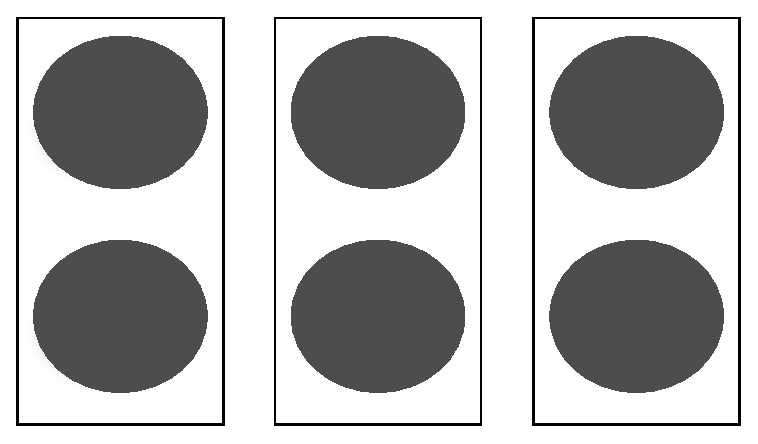
\includegraphics[scale=0.5, bb=0 0 1 1]{warizan1.eps}}
 \put(190,0){\text{図1\ :\ 3つのチーム分け}}
\end{picture}

小学校以来習ってきた割り算というのは,「たくさんあるものを,均等にチーム分けした
時のチーム数を求める演算」だと考えることができます.このイメージを
元に,「集合の割り算」を定義してみましょう.

\Section{商集合}

とはいえ,集合が与えられたとき,いきなり割り算するというのはできません.
「チーム分け」するには何が必要かを考えてみましょう.なお,大学以降では,
集合の要素のことを「元(げん)」というので,これ以降の記事では,要素を元と書くことにします.

\Subsection{同値関係}
チーム分けするためのアイディアは,「同じチームに属する条件」を与えるこ
とです.「同じチームに属している条件」を「同値関係」と言います.「同値関
係」は,以下に定義されるような3つの条件を満たす必要があります.

\begin{defi}[同値関係]
 集合$X$に対し,同値関係$\sim$とは,以下の3つの条件を満たす集合の元の間の関係をいう.
 \begin{enumerate}
  \item(反射律) 全ての$x\in X$に対し,$x \sim x.$
  \item(対称律)  $x\sim y$を満たす全ての$x,y\in X$に対し,$y\sim x$
  \item(推移律) $x\sim y$,$y\sim z$を満たす全ての$x,y,z\in X$に対し,$x\sim
	z$
 \end{enumerate}
\end{defi}
一見,難しそうな定義ですが,よく読めば大したことは言っていません.1つ目の条件は,どんな奴でも自分自身とは同じチーム,
2つ目の条件は,チームメートは逆からみてもチームメート,
3つ目の条件は,チームメートのチームメートはチームメートだと言うことです
(当然成り立ってほしい条件ですよね).


例をいくつかあげてみましょう.
\begin{Ex}
 自然数の集合$\mathbb{N}$において,元の関係$\sim$を
 \[
  n\sim m\Leftrightarrow n-mは2で割り切れる
 \]
 と定めると,これは同値関係です.実際,どんな数$n$についても,$n-n=0$は$2$で割り切れます
 し,$n-m$が$2$で割り切れるなら$m-n$も2で割り切れます.さらに,$n-m,m-l$
 が$2$で割り切れるなら$n-l$も2で割り切れます.今は「$2$」で割り切れると
 しましたが,他の自然数でも上のように定めれば同値関係になることは同様に
 示せます.
\end{Ex}


\begin{Ex}
 実数の集合$\mathbb{R}$において,$\leq(<または=)$で定められる元の関係
 \[
  x\sim y\Leftrightarrow x\leq y
 \]
 は同値関係ではありません.どんな実数$x$に対しても$x\leq x$です
 し,$x\leq y$かつ$y \leq z$ならば$x\leq z$ですから,反射律と推移律は満たしますが,対称律を満たしま
 せん.実際,$x\leq y$だからと言って,$y\leq x$とは限らないからです.
\end{Ex}

同値関係があるとき,同じチームに属している奴らを集めてきたものを,同値類と言います.例
えば,$x\in X$と同値関係にある$X$の元全体($x$が入っているチーム)を,$[x]$で書くことにします.
\[
 [x]=\{y\in X\ |\ x\sim y\}
\]
すると,集合を「チーム分け」する,つまり集合の割り算を定めることができま
す.

\Subsection{商集合の定義}

さて,同値関係が定まると集合の割り算を定義できます.

\begin{defi}[商集合]
 集合$X$とその上の同値関係
 $\sim$に対し,商集合$X/\mathord{\sim}$を以下で定める.
 \[
   X/\mathord{\sim}=\{[x]\ |\ x\in X\}
 \]
\end{defi}

例で感覚を掴みましょう.

 \begin{Ex}{\ } \\
  $X=\{0,1,2,3,4,5,6\}$とします.このとき,$X$に,同値関係$\sim$を,
 \[
  n\sim m\Leftrightarrow n-mが2で割り切れる
 \]
 と定めます.このとき,商集合$X/\mathord{\sim}$は何になるでしょうか.例えば,$1$
  の同値類($1$の入っているチーム)は,$[1]=\{1,3,5\}$, $0$の同値類は,$[0]=\{0,2,4,6\}$となります.こ
  れ以外のチームはありませんから,
  \[
    X/\mathord{\sim}=\{[0],[1]\}=\{\{0,2,4,6\},\{1,3,5\}\}
  \]
であるとわかります.まさに偶数と奇数への「チーム分け」ですよね.$\{0,1\}$
  はチームの代表メンバーであり,数学用語でも「完全代表系」と言います.しかし,
  わり算とはいえ,必ずしも1つ1つのチーム
  の元の数は一致しないことには注意しましょう.
 \end{Ex}

 \Section{様々な商集合の例}
\Subsection{合同式}
  まずは,上の概念をそのまま延長して自然数の集合$\mathbb{N}$に対して,同値
  関係$\sim$を以下で定めてみます.
  \[
   x\sim y\Leftrightarrow x-yが4で割り切れる
  \]
  この同値関係で割った集合$\mathbb{N}/\mathord{\sim}$は,4で割ったあまりでのチーム分けになり
  ます.
  \[
    \mathbb{N}/\mathord{\sim}=\{[0],[1],[2],[3]\}
  \]
  これを図にすると以下のようになります.自然数全体を4つのチームに分け
  てしまったのがよくわかると思います.\\
 \begin{picture}(200,150)(0,0)
   \put(200,20){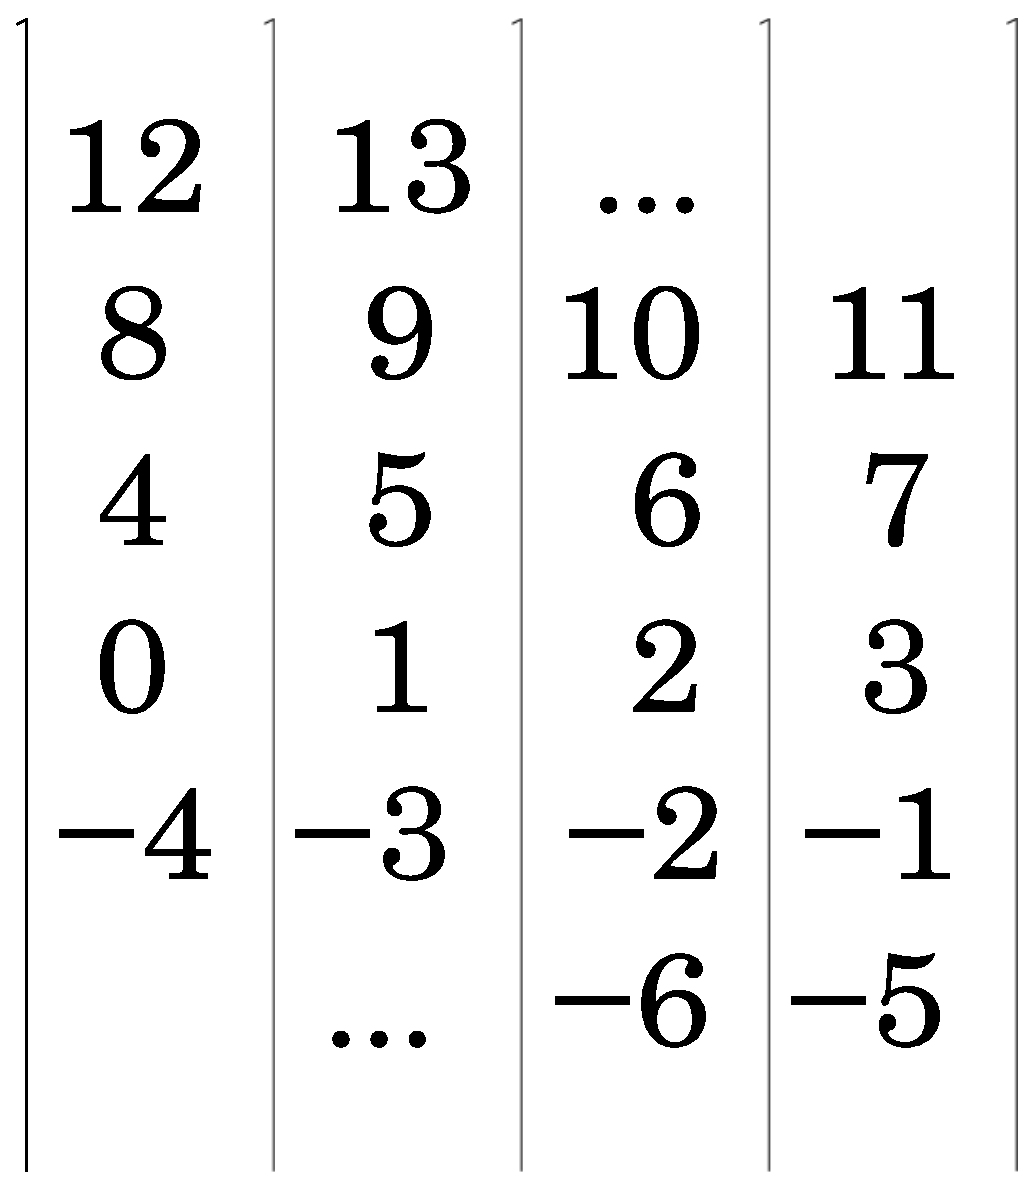
\includegraphics[scale=0.25, bb=0 0 1 1]{warizan2.eps}}
   \put(175,5){\text{図2\ :\ $4$で割ったあまりでチーム分け}}
 \end{picture}
 
  
  合同式を思い出してみましょう.
  \[
   1\equiv5  \mod4
  \]
  などという表記を見たことがあるかもしれませんが,これは,$1$と$5$が上で
  定めた同値
  関係,すなわち$1\sim 5$を示しているに他なりません.
  さらに,もともと$\mathbb{N}$に定まっている足し算,掛け算はそのまま
  $\mathbb{N}/\mathord{\sim}$に遺伝します.つまり,
  \[
   [a]+[b]=[a+b]\hspace{1cm}[a]\times[b]=[a\times b]
  \]
  が成り立つということです.これを使えば,例えば
  \[
   \bigl[15^{30}\bigr]=[15]^{30}=[3]^{30}=\bigl[3^2\bigr]^{15}=[1]^{15}=[1]
  \]
  となり,$15^{30}$がチーム$1$に属する(すなわち,4でわると1あまる)ことがすぐ確かめられます.

\Subsection{ベクトル}
今までは数字を使っていましたが,集合にしたおかげで,もっと概念的なものに
ついても商集合を考えることができます.高校で習うベクトルも,商集合として
考えてみましょう.
$E$を平面(もしくは空間)の有向線分(向きを持った線分,つまり矢印)全体から
なる集合とします.このとき,$E$上の同値関係を,
\[
 v\sim w\Leftrightarrow vとwは平行移動で重なる
\]
と定めます(同値関係になっていることはチェックしてみてください).このとき,
$E/\mathord{\sim}$がまさに平面全体のベクトルを集めた集合になります.この商集合の
 一つ一つの元は「平行移動で重なったら同じベクトルを集めたチーム」になります
 が,この中で原点を始点として持つものを「代表」とすれば,終点の「座
 標」で全てのチームが表せます.これこそがベクトルの「成分表示」なのです.

\Subsection{空間の貼り合わせ}
ベクトルの例からもわかるように,あるものたち(ベクトルの場合は平行移動し
たもの)を{\bf「おんなじものと見たい」「同一視したい」}と
いう気持ちがあるときは,商集合が使われます.数学においては図形同士を,のりで貼
り合わせたいというシーンに多々遭遇しますが,これをキチンと定式化するのも
商集合の大事な役割です.例えば,下の円と直線を黒点の部分で貼り合わせてみましょう.

\begin{picture}(150,100)(0,0)
 \put(150,10){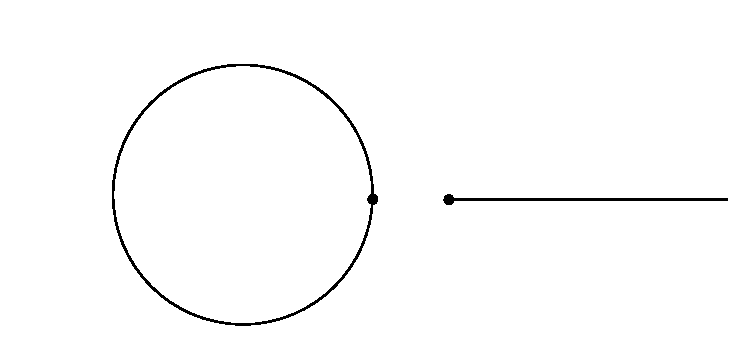
\includegraphics[scale=0.5, bb=0 0 1 1]{warizan4.eps}}
\end{picture}

このとき,二つの図形の点の集まりを一つの集合$X$だと考え,$A$を2つの黒点からなる集合として,以下のよう
な同値関係を定めます(同値関係になっていることはすぐ確かめられます).
\[
 x\sim y\Leftrightarrow 
			x,y \in Aまたは
			x=y 
\]
つまり,$A$に入っていない点たちは,その点1点からなるチームに,$A$に入っ
ている点たちはまとめて一つのチームにしてしまいます.そうすれば,チーム全
体の集合$X/\mathord{\sim}$は,まさに,二つの図形を貼り付けたものになっていることがわかりま
す.
このような貼り付けにより作られる図形の一つをみてみましょう.正方形の辺を貼り付けて立体を作るということを考えてみます.図の黒点同士のように,左側の辺と右
側の辺,上と下も同様に,同じ方向に貼り付けると,右のように浮き輪の形の図
形が出来上がります.これは(2次元)トーラスといい,数学の様々な場面に登場
します.

\begin{picture}(400,120)(0,0)
 \put(40,10){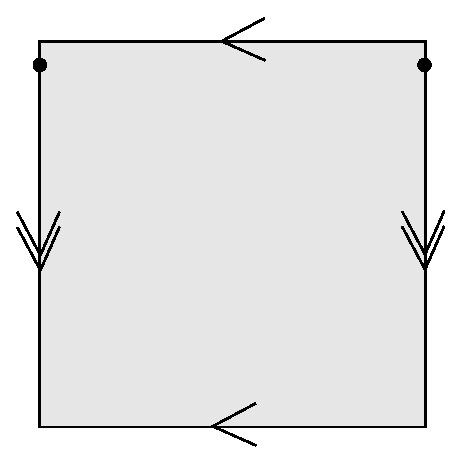
\includegraphics[scale=0.5, bb=0 0 1 1]{warizan3.eps}}
 \put(150,55){\text{\huge $\Rightarrow$}}
 \put(175,30){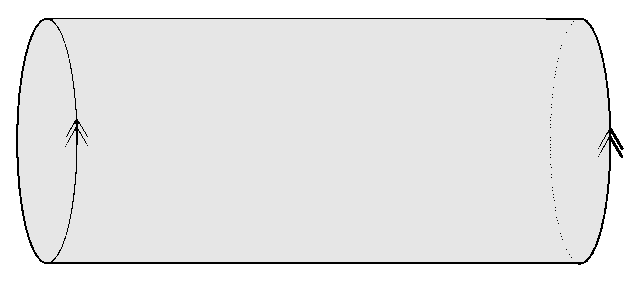
\includegraphics[scale=0.5, bb=0 0 1 1]{warizan5.eps}}
 \put(325,55){\text{\huge $\Rightarrow$}}
 \put(350,30){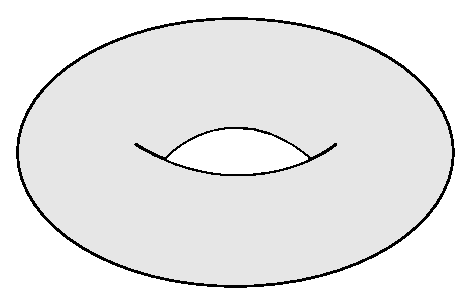
\includegraphics[scale=0.5, bb=0 0 1 1]{torus.eps}}
 \end{picture}

ちなみに,貼り付けかたを一つだけ逆にすればクラインの壺,二つとも逆に
すると二次元射影空間と呼ばれる図形になります(想像できますか?).\\
二次元球面(地球の表面)は地球上の地図を貼り合わせて構成できますし,多くの図形は
貼り合わせによって構成が可能です.大雑把に言って,このように直線や平面な
どまっすぐな空間を貼り合
わせて作られる図形のことを数学では多様体と呼び,古くから研究されてきた対
象です.

\Subsection{商ベクトル空間*}
ここで扱う例は,大学1年生で習うベクトル空間の概念なので,知らない人は
飛ばしてもらって結構です.\\

ここまでの概念がわかってしまえば,大学1年生の線形代数での1つの難所である
商空間は簡単に定義できます.

\begin{defi}
 ベクトル空間$V$と部分空間$W$に対し,$V$上の同値関係を,
 \[
  v_1\sim v_2\Leftrightarrow v_1-v_2\in W
 \]
 と定義する.$V/\mathord{\sim}$を,部分空間$W$による$V$の商空間といい,$V/W$で表す.
\end{defi}

これだとイメージしにくいかもしれませんが,$v_1$の同値類$[v_1]$は
$v_1+w\ (w\in W)$
と書けるものな訳ですから,$W$の元だけずれているものは全て同じチームなの
です.絵で描けば,以下のようになります.まず,部分空間とは,原点を通るまっ
すぐな空間ですから,$V$と$W$の図は以下のようになります.\\
\begin{picture}(400,150)(0,0)
 \put(150,10){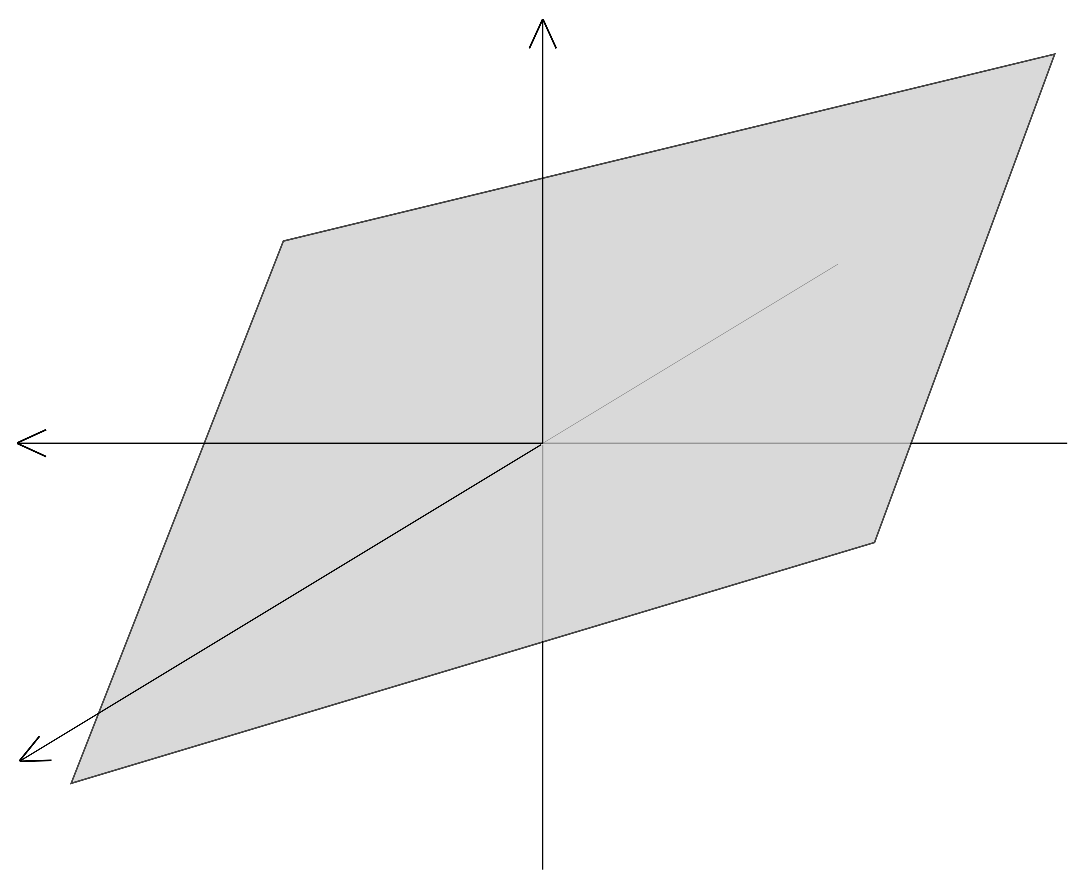
\includegraphics[scale=0.4, bb=0 0 1 1]{warizan6.eps}}
 \put(260,100){\text{$W$}}
\end{picture}

この空間$W$全てが同じチームとなりますので,チームは以下
のようにならんでいることがわかります.つまり,商空間とは,この1枚1枚のチームの全体となるの
です.完全代表系は,$W$と原点のみにおいて交わる直線と平面たちの交点となり
ます(完全代表系の取り方は無限通りあります).つまり,商空間$V/W$はこの直線と同
一視できるのです.スカラー倍や足し算については合同式のときと同じく商集合に遺
伝することが示せるので,$V/W$もベクトル空間となることがわかります.
イメージとしては,商空間$V/W$は$V$を図の直線に向かって潰した空間というこ
とになります.潰した時,$W$は原点に潰れるわけですから,$V$において,$W$
の成分を全て$0$と同一視したものだとも言えます.


\begin{picture}(400,150)(0,0)
 \put(150,10){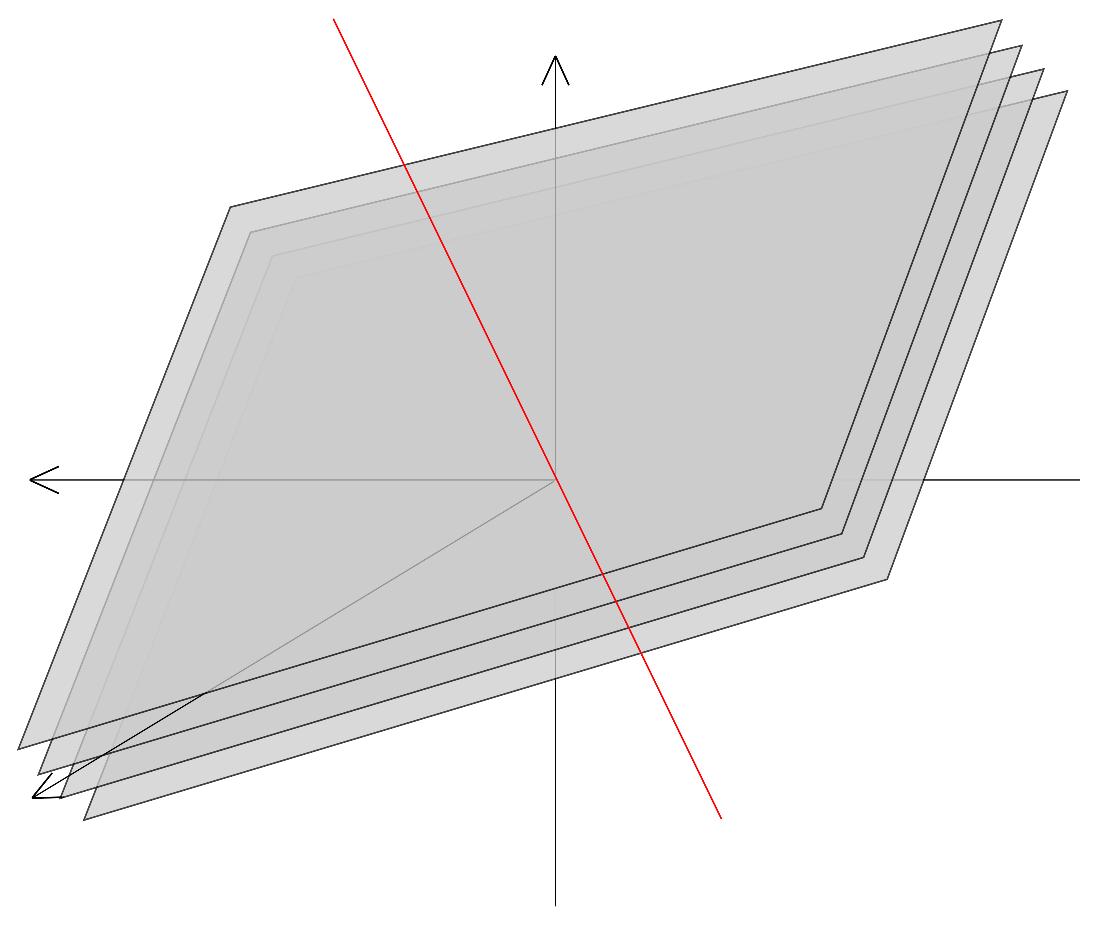
\includegraphics[scale=0.4, bb=0 0 1 1]{warizan7.eps}}
\end{picture}
\Section{数の構成}

さて,ここからは応用編です.唐突ですが,「整数,有理数,実数とは何か」と聞かれ
たとき,何て答えるでしょうか.「え,そりゃあ,$-1$とか分数とかでしょ?」
とか答えられても,あくまでそれは例にすぎません.「自然数の集合
$\mathbb{N}$と足し算,掛け算しか知らない」と仮定
して,整数の集合$\mathbb{Z}$や有理数の集合$\mathbb{Q}$,実数の集合$\mathbb{R}$を自然数のみを用いて構成してみ
ることにします.(今回は,自然数の存在は暗に認めています.公理的集合論の
立場では自然数は無限公理を満たす最小の集合として存在を保証しているのですが,今回は解説しないことにし
ます.)\footnote{以下の話の厳密な証明が知りたい場合,\cite{mathpdf}を参照してください.}

\Subsection{自然数から整数}

さて,自然数から整数を構成することを考えてみましょう.一番簡単なアイディ
アは,プラスパートとマイナスパートの自然数を作るということです.$(a,b)$と書
いたとき,1つめの項はプラス,2つ目の項はマイナスに当たると考えてみましょ
う.例えば,$(2,0)$を$2$に当たる数として,$(0,3)$を$-3$に当たる数として定めるわけです.そして,2つの数
の足し算を$(2,0)+(0,3)=(2,3)$と定めます.$(2,3)$はプラスパートとマ
イナスパートがそれぞれ$2,3$ですから,$-1$を表していると考えます.これで一見,うまくいっ
たかのように見えますが,これだと$(2,3)$と$(0,1)$が同じ数字を表しているた
め,”ダブり”が生じています.$(2,3)$と$(0,1)$を同じものと見たい,同一視し
たい.こんな時こそ商集合の出番です.


\begin{defi}[整数]
 自然数を二つ並べた集合$\mathbb{N}^2=\{(a,b)\ |\ a,b\in
\mathbb{N}\}$を考え,$\mathbb{N}^2$上に同値関係
\[
 (a,b)\sim(c,d)\Leftrightarrow a+d=b+c
\]
と定め,この同値関係による商集合$\mathbb{N}/\mathord{\sim}$を整数$\mathbb{Z}$と
 定める.
 さらに,$\mathbb{Z}$上の加法と乗法を,
 \[
  [(a,b)]+[(c,d)]=[(a+b,c+d)]\hspace{1cm}[(a,b)]\times[(c,d)]=[(ac+bd,ad+bc)]
 \]
 と定める\footnote{本当は,これで矛盾なく定まっていることをチェックしなければいけません.つまり,$(a,b)\sim(a',b')$のとき,\[(a+c,b+d)\sim(a'+c,b'+d)\hspace{1cm}(ac+bd,ad+bc)\sim(a'c+b'd,a'd+b'c)\]であることを示す必要があります.もしこうでなければ,足し算や掛け算の結果が,チームの代表メンバーの選び方によって違う結果になってしまい,矛盾してしまうからです.一つ目だけチェックすれば,$a+b'=a'+b$より$(a+c)+(b'+d)=(a'+c)+(b+d)$ですからうまくいっています(二つ目もチェックしてみましょう).このようにうまく定まっていることを,数学では,well-definedと言います.}
\end{defi}

例えば,$2+1=3+0$ですから,$[(2,3)]=[(0,1)]$だとわかりま
す.
掛け算はちょっと技巧的ですが,これでうまくいっていることがわかります.例
えば,正の数同士は,$[(n,0)]\times[(m,0)]=[(nm,0)] $と,今までと全く同じ
演算であることがわかります.また,$[(n,0)]\times[(0,m)]=[(0,nm)]$や,
$[(0,n)]\times[(0,m)]=[(nm,0)]$などから,プラスかけるマイナスがマイナ
ス,マイナスかけるマイナスがプラスであることも説明できます.\\
最後に,$[(x,0)]$を$x$とかき,$[(0,x)]$を$-x$を書くことにすれ
ば,今まで使っていた表記と合致します.


\Subsection{整数から有理数}

さて,今度は有理数を構成してみましょう.さっきのアイディアをそのまま借用
して,分母パートと分子パートを並べて書いてみることにします.つまり,
$(a,b)$と書いたとき,$\ds\frac{a}{b}$を表すとしてみます.しかし,分数と
いうのは,小学校以来,約分しても同じ,だったわけですから,例えば$(2,4)$
と$(1,2)$は同じものであってほしいわけです.そこで,商集合を使って同一視
してみます.

\begin{defi}[有理数]
$\mathbb{Z}\times(\mathbb{Z}-\{0\})=\{(a,b)\ |\
 a\in\mathbb{Z},b\in\mathbb{Z}-\{0\}\}$上に同値関係
 \[
  (a,b)\sim(c,d)\Leftrightarrow ad=bc
 \]
 と定め,この同値関係による商集合
 $\mathbb{Z}\times(\mathbb{Z}-\{0\})/\mathord{\sim}$を有理数$\mathbb{Q}$と定める.
 さらに,$\mathbb{Q}$上の加法と乗法を,
 \[
  [(a,b)]+[(c,d)]=[(a+c,b+d)]\hspace{1cm}[(a,b)]\times[(c,d)]=[(ac,bd)]
 \]
 と定める\footnote{これもwell-definedであることをチェックする必要があります.示してみてください.}.
\end{defi}

$\sim$の同値関係は,外項と内項の積が等しい,つまり,$a:b=c:d$を表していますから,同じ分数を1チームにまとめていることがわかります.\\
さて,定義から,$[(1,1)]$はどんな数とかけても相手を変えない,自然数の''1''に当たる数だとわかります.また,$[(0,1)]$は,どんな数とかけても$[(0,1)]$になり,どんな数と足し算しても相手を変えない,自然数の''0''に当たる数だとわかります.\\
また,
\[
 [(a,b)]\times[(b,a)]=[(ab,ab)]=[(1,1)]
\]
ですから,$[(a,b)]$に,$[(b,a)]$をかけると1になることがわかります.
ということは,
\[
 [(c,d)]=[(a,b)]\times([(b,a)]\times[(c,d)])
\]
ですから,
\[
 [(c,d)]/[(a,b)]=[(b,a)]\times[(c,d)]
\]
となり,小学校以来やってきた,分数の割り算は分母と分子をひっくり返してかけるということも正当化できます.

最後に,$(a,b)$を$\ds\frac{a}{b}$と書く\footnote{ちなみに,$\ds\frac{a}{b}$は日本語では「$b$分の$a$」と読みますが,英語では逆で,''$a$ over $b$''と読みます.}ことにすれば,今まで使っていた表記と合致します.

\Subsection{有理数から実数}

さて,最後に実数を作ってみましょう.これはかなり困難です.実数の構成には,代表的なものでDedekint cutによるものと,有理数の完備化の二つがあるのですが,今回は有理数の完備化を解説したいと思います.
\begin{defi}[Cauchy列]
 数列$\{a_n\}$がCauchy列であるとは,以下のことを言う.
 \[
  \forall \varepsilon >0 \ \exists N\  {\rm such\ that}\ n,m>N \Rightarrow |a_n-a_m|<\varepsilon
 \]
\end{defi}
一見ギョッとするような定義ですが,簡単に言えば,コーシー列とは,「二項間の差がどんどん小さくなっていくような数列」のことです.
さて,ここで,次のような問題を考えて見ましょう.
\begin{center}
 Cauchy列は収束するでしょうか?
\end{center}
答えは,実数列なら○,有理数列なら×です.数学用語でこの性質を「完備性」と言います.有理数は完備ではないのです.例えば,有理数で$\sqrt{2}$に近づくような数列を考えてみれば,もちろん二項の差は縮まっていきますが,肝心の収束先の$\sqrt{2}$が有理数ではないですから,「有理数の中では」収束しません.このことに着目して,有理数から実数を作ります.具体的には,
\begin{center}
  $\sqrt{2}$ に収束する有理数列を $\sqrt{2}$ だと定義する
\end{center}
です.数列と $\sqrt{2}$ を同じと見るなんてかなり気持ち悪いですが,一応定義はできるわけです.とはいっても,$\sqrt{2}$に収束する有理数列はいっぱいあります.そこで,商集合の考え方を使って,$\sqrt{2}$に収束する数列を1チームにしてしまえば良いのです.
\begin{defi}[実数]
$\mathcal{C}$を有理数のCauchy列全体からなる集合とし,$\mathcal{C}$上の同値関係を,
 \[
 \{a_n\}\sim\{b_n\}\Leftrightarrow \forall\varepsilon\  \exists N\  {\rm such\ that}\ n>N\Rightarrow |a_n-b_n|<\varepsilon
 \]
 と定め\footnote{これが同値関係であることは非自明ですが,ここでは省略します.},この同値関係による商集合$\mathcal{C}/\mathord{\sim}$を実数$\mathbb{R}$と定める.さらに,$\mathbb{R}$上の加法と乗法を,
 \[
  [\{a_n\}]+[\{b_n\}]=[\{a_n+b_n\}]\hspace{1cm}[\{a_n\}]\times[\{b_n\}]=[\{a_nb_n\}]
 \]
 と定める.\footnote{これがwell-definedであることも非自明ですが,ここでは省略します.}
\end{defi}

上のように定めれば$\{a_n\}\sim\{b_n\}$であれば,$\{a_n\}$と$\{b_n\}$が同じ値に近づいていくことがわかります.
本当は,$\mathbb{R}$が満たすべきたくさんの性質をここから示さなければいけないのですが,今回の主題はそこではないので,詳しくは参考文献を見てみてください.

このように,存在が当たり前だと思っていた整数や有理数や実数,そしてそのたくさんの性質は,商集合のアイディアに支えられているのです.\footnote{実は複素数も,商集合を用いて$k[X]/(X^2+1)$などと定義できるのですが,今回は紙面の関係上,省略します.}


\Section{応用**}
最後に,少しだけ応用をみてみます.
 \Subsection{等質空間}
群構造をもつ可微分多様体で群の積演算$(a,b)\mapsto ab$と逆演算$a\mapsto a^{-1}$が可微分であるものをLie群と言います(群と多様体のあいのこです).例えば,一般線形群$GL(n,\mathbb{R})$や特殊線形群$SL(n,\mathbb{R})$,特殊直交群$SO(n)$などはLie群になっています.

さて,Lie群$G$がある多様体$M$に推移的に作用していることを考えてみましょう.推移的,というのは全ての点同士があるLie群の元の作用で写りあえるという意味です.全射群準同型$G\rightarrow \rm{Diff}(M)$があると言ってもいいです.
例えば,球面$S^n$,上半平面$H$には,
\begin{eqnarray*}
SO(n+1)&\rightarrow & {\rm Diff}(S^{n})\hspace{1cm}A\mapsto (p\mapsto Ap)  \\
SL(2,\mathbb{R})&\rightarrow & {\rm Diff}(H)\hspace{1cm}\left(\begin{matrix}a&b\\c&d\end{matrix}\right)\mapsto\left(z\mapsto\frac{az+b}{cz+d} \right) 
 \end{eqnarray*}
のように,Lie群が推移的に作用しています.
この時,ある一点$p$の群作用による行き先(軌道)は,推移的であるという仮定から全体を覆うわけですが,作用させても動かない$G$の元があるかもしれません.これを集めたもの,
\[
 H=\{g\in G\ |\ gp=p\}
\]
を$G$の一点$p$の固定部分群と言います(定義より閉部分群になります).
この$H$たちをチームにして, 点$p$と同一視すれば,作用させている空間との1対1対応ができます.
すなわち,
\[
 G/H\simeq M\hspace{1cm}[g]\mapsto gp
\]
となるわけです.

ここで,左辺の$G/H$とは,$G$を,$g_1\sim g_2\Leftrightarrow g_1g_2^{-1}\in H$という同値関係で割ったもので,$G$の部分群$H$による商群と呼ばれます.特に,Lie群をその中の閉部分群で割った商群$G/H$には多様体構造が定まることが知られており,上の同型は微分同相であることが示せます.

このように,Lie群が推移的に作用している多様体は,必ずLie群の商の形で書くことができます.このような多様体を等質空間と言います.

\begin{Ex}[球面]
 $SO(n+1)$の作用による球面$S^n$上のある1点$(0,0,0,\cdots,0,1)$の固定部分群は,
 \[
\left\{
\left(
\begin{array}{ccc:c}
&&&\\
&\mbox{\smash{\huge\textit{A}}}&&{{0}}\\
&&&\\ \hdashline
&0&&1
\end{array}
\right) \middle|\ A\in SO(n) \right\}\simeq SO(n)
 \]
よって,$S^n\simeq SO(n+1)/SO(n)$となります.
\end{Ex}

\begin{Ex}[上半平面]
$SL(2)$の作用による上半平面$H$上のある1点 $i$ ($=\sqrt{-1}$) の固定部分群は,
 \[
  \frac{ai+b}{ci+d}=i\Leftrightarrow a=d,\ b=-c
 \]
より,
 \[
  \left\{\left(\begin{matrix}
   a&b\\c&d
  \end{matrix}\right)\in SL(2,\mathbb{R})\ \middle|\  a=d,b=-c\right\}\simeq SO(2)
 \]
よって,$H\simeq SL(2,\mathbb{R})/SO(2)$となります.$H$は複素多様体ですが,実Lie群の商でかけます.
\end{Ex}

この表示の一つのメリットは,ある1点に定めた幾何構造を全体に写すことにあります.
$G/H$の形で書いた場合,当然,原点の同値類$[e]$があります.
これについて
\begin{Lemma}\label{l4}
  $G/H$を等質空間とする.集合として,次の同型がある.
 \[
  (\bigotimes^rT_{[e]}M\otimes\bigotimes^sT^*_{[e]}M)^H\simeq (\Gamma(M,\bigotimes^rTM\otimes\bigotimes^sT^*M))^G
 \]
 ただし,左は,$\Ad(H)$不変なテンソルの元,右辺は$M$からベクトル束への左作用の微分${L_{G}}_*$不変な切断である.
 \end{Lemma}
表示は仰々しいですが,例えば,$r=1,s=0$とすれば,$H$不変な接空間のベクトルと,$G$不変なベクトル場が1対1に対応していることがわかりますし,$r=0,s=2$とすれば,$H$不変な接空間上の内積と,$G$不変な計量,$H$不変な複素構造と$G$不変な概複素構造が1対1に対応することがわかります.\\
他にも,等質空間上では測地線をLie代数からLie群への指数写像でかけたり,曲率テンソルが,Lie括弧でかなりシンプルにかけたりなど,計算できる具体例を豊富に提供してくれます.


\Subsection{Clifford-Klein形}
Riemannの一意化定理の一般化である,Klein-Poincar\'e-Koebeの一意化定理より,Riemann面の普遍被覆は,上半空間$H$,複素数$\mathbb{C}$,複素射影空間$\mathbb{P}^1$のいずれかに正則同値になります.また,特に,種数が2以上のコンパクトRiemann面は,上半平面を,Fuchs群と呼ばれる$\rm{Aut}(H)$の離散部分群$\Gamma$で割って作られます.$H$自体は上で見たように$SL(2,\mathbb{R})/SO(2)$とかけますから,コンパクトRiemann面は,$\Gamma\backslash SL(2,\mathbb{R})/SO(2)$という$SL(2,\mathbb{R})$を2回割ったものとして書くことができます.一般に,$G/H$に固有不連続かつ自由に作用する$G$の離散部分群$\Gamma$が存在すれば,等質空間$G/H$をさらに割った$\Gamma\backslash G/H$を考えられます.これをClifford-Klein形といい,等質空間より豊富な例を含む広いクラスとして,現在も研究されています.

{\bf 終わりに}\\
たくさんの例を「割り算」というテーマでざっくばらんに解説してみました.何を隠そう,この集合の割り算という概念を理解するのに僕自身苦労したので,あえて書いて見ました.数学というと,「イメージではなく,論理的にのみ考える学問」と考えられがちな気がします.論理ももちろん大事ですが,決して論理だけではなく,むしろ,「イメージをいかに数式という形で正確に伝えられるか」というモチベーションで研究が進むことも多いと思います.高校や大学で難しい概念に出会ったときは,ただ定義を眺めるだけではなく,様々な例を見ながら,どういう気持ちで概念が生まれているのかを考えて見るといいと思います.

\begin{thebibliography}{99}
\bibitem{mathpdf} 数の構成 自然数から複素数まで \url{http://mathematics-pdf.com/pdf/construction_of_numbers.pdf}
\bibitem{hel} S.Helgason.Differetntail Geometory and Symmetric Spacees.AMS Chelsea Publishing,2001
\bibitem{sat} 佐武一郎.線型代数学.裳華房,数学選書1,1974
\bibitem{mat} 松坂和夫.集合・位相入門.岩波書店,1968
\bibitem{kob} 小林俊行.数学の最先端21世紀への挑戦.vol1.Springer,2001
\end{thebibliography}
%\documentclass{ltjsarticle}
%\usepackage{luatexja-ruby}
%\usepackage{amsmath,amssymb,amsthm}
%\usepackage[unicode]{hyperref}
{
\newcommand{\Natural}{\mathbf{N}}
\newcommand{\Rational}{\mathbf{Q}}
\newcommand{\Complex}{\mathbf{C}}

\renewcommand{\equationautorefname}{式}
\newtheorem{theorem}{定理}
\renewcommand{\theoremautorefname}{定理}
\newtheorem*{example*}{例}

\newaliascnt{remark}{theorem}
\newtheorem{remark}[remark]{注意}
\aliascntresetthe{remark}
\newcommand{\remarkautorefname}{注意}

\newaliascnt{lemma}{theorem}
\newtheorem{lemma}[lemma]{補題}
\aliascntresetthe{lemma}
\newcommand{\lemmaautorefname}{補題}

\newaliascnt{proposition}{theorem}
\newtheorem{proposition}[proposition]{命題}
\aliascntresetthe{proposition}
\newcommand{\propositionautorefname}{命題}

\newaliascnt{corollary}{theorem}
\newtheorem{corollary}[corollary]{系}
\aliascntresetthe{corollary}
\newcommand{\corollaryautorefname}{系}

\newcommand{\stirlingI}{\genfrac[]{0pt}{}} % 第1種スターリング数
\newcommand{\stirlingII}{\genfrac\{\}{0pt}{}} % 第2種スターリング数
\newcommand{\risingFactorial}[2]{{#1}^{\overline{#2}}}
\newcommand{\fallingFactorial}[2]{{#1}^{\underline{#2}}}

\renewcommand{\proofname}{証明}

\Chapter{ベルヌーイ数小噺(荒田)}

前半は高校生程度の知識で読める。後半は複素関数の知識が必要となる。

\section{自然数のべき乗の和}
自然数のべき乗の和は、次のように $n$ の多項式で書ける。
高校では次の3つを学ぶはずだ:
\begin{align*}
  1+2+\dotsb+n&=\sum_{k=1}^n k=\frac{n(n+1)}{2}, \\
  1^2+2^2+\dotsb+n^2&=\sum_{k=1}^n k^2=\frac{n(n+1)(2n+1)}{6}, \\
  1^3+2^3+\dotsb+n^3&=\sum_{k=1}^n k^3=\frac{n^2(n+1)^2}{4}.
\end{align*}
では、4乗の和や5乗の和を表す公式はどうなるか?
もっと言うと、自然数 $p$ について $k^p$ の和を表す一般的な式はあるか?

先に答えを述べると、自然数の $p$ 乗の和(以後これを、ここだけの記号で $s_p(n)$ とおく)は $n$ についての $p+1$ 次の多項式であり、有理数の数列 $B_k$ ($k=0,1,2,\dotsc$) を使って次のように書ける:
\[
  s_p(n)=\sum_{k=1}^n k^p=\frac{1}{p+1}\sum_{k=1}^{p+1} \binom{p+1}{k} (-1)^k B_k n^{p+1-k}
\]
この $B_k$ はベルヌーイ数(Bernoulli numbers)と呼ばれる数列で、最初の数項は次のようになる:
\[
  B_0=1,\
  B_1=-\frac12,\
  B_2=\frac16,\
  B_3=0,\
  B_4=-\frac{1}{30},\
  B_5=0,\dotsc
\]
ベルヌーイ数は次の初項と漸化式によって計算できる:
\begin{align*}
  B_0&=1, \\
  B_n&=-\frac{1}{n+1}\sum_{k=0}^{n-1} \binom{n+1}{k} B_k
\end{align*}
ベルヌーイ数は文献によって符号が若干違っていたり、奇数番目を飛ばしていたりするので、文献ごとに定義を確認するようにしたい。

\subsection{自然数のべき乗の和の公式の導出}
まず、 $p$ が自然数のとき、 $s_p(n)$ は $n$ についての $p+1$ 次の多項式である\footnote{%
証明のやり方はいくつかあるが、詳細は割愛する。
一つのやり方としては、
\[(k+1)^{p+1}-k^{p+1}=(p+1)k^p+\dotsb+(p+1)k+1\]
を $k=1,\dotsc,n$ について辺ごとに足すというものがある。
別のやり方を\ref{sec:stirling-numbers} で与える。
}。
そこで、 $n^{p+1-k}$ の係数を $a_k$ とおき、
\[
  s_p(n)
  =a_0 n^{p+1}+a_1 n^p+\dotsb+a_{p} n+a_{p+1}
  =\sum_{k=0}^{p+1} a_k n^{p+1-k}
\]
と書く。

さて、 $s_p(n)$ は次の2つの式を満たす:
\begin{align}
  s_p(0)&=0, \label{eq:s_p-at-zero} \\
  \forall n\in\Natural.\ s_p(n)-s_p(n-1)&=n^p. \label{eq:s_p-inductive-definition}
\end{align}
逆に、これらの式を満たす多項式があれば、その多項式は $s_p(n)$ と一致する。

ちなみに、$s_p(n)$ が多項式であることに留意すれば、2番目の式を多項式としての等式
\begin{equation*}
  s_p(x)-s_p(x-1)=x^p
\end{equation*}
としても同じことになる。

\autoref{eq:s_p-at-zero} と\autoref{eq:s_p-inductive-definition} から、係数 $a_k$ に対する何らかの条件が得られるはずである。
まず、\autoref{eq:s_p-at-zero} からは $a_{p+1}=0$ がわかる。

\autoref{eq:s_p-inductive-definition} については、左辺を $a_i$ によって表すと
\begin{align*}
  s_p(n)-s_p(n-1)
  =&\sum_{i=0}^{p+1} a_i n^{p+1-i}-\sum_{i=0}^{p+1} a_i (n-1)^{p+1-i} \\
  =&\sum_{i=0}^{p+1} a_i n^{p+1-i}-\sum_{i=0}^{p+1} a_i \sum_{j=0}^{p+1-i} \binom{p+1-i}{j} (-1)^j n^{p+1-i-j} \\
  %& (\text{途中計算は各自で}) \\
  % m = i+j, k=i, j=m-l
  =&\sum_{i=0}^{p+1} a_i n^{p+1-i}-\sum_{m=0}^{p+1} \sum_{k=0}^{m} \binom{p+1-k}{m-k} (-1)^{m-k} a_l n^{p+1-m} \\
  %=&\sum_{i=0}^{p+1} \left(a_i-\sum_{k=0}^{i} \binom{p+1-k}{i-k} (-1)^{i-k} a_k\right) n^{p+1-i} \\
  =&\sum_{i=1}^{p+1} \left(\sum_{k=0}^{i-1} \binom{p+1-k}{i-k} (-1)^{i-k-1} a_k\right) n^{p+1-i}
\end{align*}
となる。ただし、 $\binom{n}{k}:=\frac{n!}{(n-k)!k!}$ は二項係数である\footnote{高校では ${}_n C_k$ というような記号で書くかもしれない。}。

つまり、\autoref{eq:s_p-inductive-definition} を $a_i$ の言葉で書けば、
\[
  n^p=\sum_{i=1}^{p+1} \left(\sum_{k=0}^{i-1} \binom{p+1-k}{i-k} (-1)^{i-k-1} a_k\right) n^{p+1-i}
\]
となる。この両辺の $n^{p+1-i}$ の係数を比較することにより、
\begin{align}
  1&=(p+1)a_0 & (i&=1) \notag \\
  0&=\sum_{k=0}^{i-1} \binom{p+1-k}{i-k} (-1)^{i-k-1} a_k & (1&<i\le p+1) \label{eq:a_k-inductive-formula}
\end{align}
を得る。\autoref{eq:a_k-inductive-formula} を変形すると
\begin{align*}
  0&=\sum_{k=0}^{i-1} \binom{p+1-k}{i-k} (-1)^{i-k-1} a_k \\
   %&=(-1)^{i-1}\sum_{k=0}^{i-1} \frac{(p+1-k)!}{(i-k)!(p+1-i)!} (-1)^{k} a_k \\
   &=(-1)^{i-1}\frac{(p+1)!}{i!(p+1-k)!}\sum_{k=0}^{i-1} \frac{i!}{k!(i-k)!}\frac{k!(p+1-k)!}{(p+1)!} (-1)^{k} a_k \\
   %&=(-1)^{i-1}\sum_{k=0}^{i-1} \binom{i}{k}\binom{p+1}{i}\left.(-1)^{k} a_k \middle/\binom{p+1}{k}\right. \\
   &=(-1)^{i-1}\binom{p+1}{i} \sum_{k=0}^{i-1} \binom{i}{k}\left.(-1)^{k} a_k \middle/\binom{p+1}{k}\right.
\end{align*}
となり、結局 $1<i\le p+1$ について
\[
  0=\sum_{k=0}^{i-1} \binom{i}{k}\left.(-1)^{k} a_k \middle/\binom{p+1}{k}\right.
\]
を得る。
ここで、やや天下り的\footnote{%「天下り的」の意味を説明する
理由や出どころを隠して式や定義をどこからともなく持ってくることを「天下り的」である、という。
例えば、$\alpha$ が方程式の解だと知っている人が「方程式に $\alpha$ を代入したら成立するから解の1つは $\alpha$ だ!」という議論をした場合、これは天下り的である。
本文中の用例では、筆者の心の中には「このように $B_k$ を定義すれば漸化式が綺麗になるし、世間でいうベルヌーイ数の定義と一致する」という気持ちがあるわけだが、それを本文に書いていないので「天下り的」である。
}だが、新たに記号 $B_k$ を導入して $a_k$ を
\begin{equation} \label{eq:bernoulli-number-and-coefficient}
  a_k=\frac{(-1)^{k}}{p+1}\binom{p+1}{k}B_{k} \qquad (0\le k\le p)
\end{equation}
と置くことにする。すると、$B_k$ は
\begin{align}
  B_0&=1, \notag \\
  0&=\sum_{k=0}^m \binom{m+1}{k} B_k \qquad (1\le m) \label{eq:bern-inductive-formula}
\end{align}
を満たす。\autoref{eq:bern-inductive-formula} を $B_m$ に関して解くと
\[
  B_m=-\frac{1}{m+1}\sum_{k=0}^{m-1} \binom{m+1}{k} B_k\qquad (1\le m)
\]
という漸化式が得られる。
この初項と漸化式は $p$ に依存しないので、 $B_k$ は $p$ によらない数列である。
この $B_k$ こそが、冒頭に書いたベルヌーイ数である。

結局、$s_p(n)$ は、ベルヌーイ数によって
\begin{equation} \label{eq:s_p-with-bernoulli-numbers}
  s_p(n)=\frac{1}{p+1}\sum_{k=0}^{p} \binom{p+1}{k} (-1)^{k} B_{k} n^{p+1-k}
\end{equation}
と書ける。

\subsection{べき乗和の公式の性質}
以下、 $s_p(x)$ の多項式としての性質をいくつか見ていく。

\begin{theorem} \label{thm:s_p-reflection}
  $p\ge 1$ のとき、
  $s_p(-x)=(-1)^{p+1}s_p(x-1)$.
\end{theorem}
\begin{proof}
  自然数 $n$ を任意に取ったとき、
  \begin{align*}
    s_p(0)-s_p(-n)
    &=\sum_{k=-n+1}^{0} (s_p(k)-s_p(k-1)) \\
    &=\sum_{k=-n+1}^{0} k^p
     =0^p+(-1)^p+(-2)^p+\dotsb+(-n+1)^p \\
    &=(-1)^p s_p(n-1)
  \end{align*}
  より、
  \[s_p(-n)=(-1)^{p+1} s_p(n-1)\]
  が成り立つ。
  この等式は全ての自然数 $n$ について成り立つので、 $s_p(-x)$ と $(-1)^{p+1} s_p(x-1)$ は多項式として等しい。
  (この証明は $0^p=0$ となることに依存しているので、 $p=0$ の時は成り立たない)
\end{proof}

\begin{corollary} \label{thm:s_p-minus1/2}
  $p$ が $2$ 以上の偶数のとき、
  $s_p\bigl(-\frac12\bigr)=0$.
  特に、$s_p(x)$ は $p$ が $2$ 以上の偶数のとき $2x+1$ で割り切れる。
\end{corollary}

\begin{theorem}[Faulhaber] \label{thm:Faulhaber}
  $p$ が奇数のとき、 $s_p(x)$ は $s_1(x)=\frac{x(x+1)}{2}$ の多項式として書ける。

  $p$ が $2$ 以上の偶数のとき、 $\frac{s_p(x)}{x+1/2}$ は $s_1(x)$ の多項式として書ける。
\end{theorem}
\begin{proof}
  $p$ が奇数の場合は、\autoref{thm:s_p-reflection} および、後に述べる\autoref{lem:skew-symmetric-polynomial} より従う。

  $p$ が2以上の偶数のときは、 $s_p(x)$ は $2x+1$ で割り切れる(\autoref{thm:s_p-minus1/2})ので、 $\frac{s_p(x)}{x+1/2}$ は多項式である。
  $f(x)=\frac{s_p(x)}{x+1/2}$ と置いたときに $f(-x)=f(x-1)$ が成り立つことを示して、\autoref{lem:skew-symmetric-polynomial} を使えば良い。
\end{proof}

\begin{lemma} \label{lem:skew-symmetric-polynomial}
  多項式 $f(x)$ が $f(-x)=f(x-1)$ を満たすならば、 $f(x)$ は $s_1(x)=\frac{x(x+1)}{2}$ の多項式として書ける。
\end{lemma}
\begin{proof}
  $\Rational[x]$ の部分集合 $V$ を $V=\{f\in\Rational[x]\mid f(-x)=f(x-1)\}$ により定める。
  \autoref{thm:s_p-reflection} より、 $s_p$ は $V$ の元である。
  $V$ の元は全て $s_1(x)$ の多項式として書けることを、 $V$ の元 $f$ の次数に関する帰納法で示す。

  $\deg f=0$ の場合はOK。
  $\deg f=1$ の場合は $f(-x)=f(x-1)$ とはなり得ないので考える必要はない。

  $\deg f\ge 2$ の場合。
  写像 $F\colon V\to V$ を
  \[Ff(x):=\frac{f(x)-f(0)}{x(x+1)/2}\]
  により定める。
  多項式 $f(x)-f(0)$ は $x(x+1)$ で割り切れるので、 $Ff$ は多項式である。
  $Ff\in V$ は
  \[Ff(-x)=\frac{f(-x)-f(0)}{(-x)(-x+1)/2}=\frac{f(x-1)-f(0)}{x(x-1)/2}=Ff(x-1)\]
  とわかる。
  定義より、 $\deg Ff<\deg f$ なので、帰納法の仮定より、 $Ff$ は $s_1$ の多項式として書ける。
  \[f(x)=f(0)+\frac{x(x+1)}{2}Ff(x)\]
  より、$f$ も $s_1$ の多項式である。
\end{proof}

\begin{example*}
  $S=x(x+1)/2$ とおくと、
  \begin{align*}
    s_3(x)&=S^2, \\
    s_4(x)&=\frac{(2x+1)(6S^2-S)}{15}, \\
    s_5(x)&=\frac{S^2(4S-1)}{3}.
  \end{align*}
\end{example*}

\begin{theorem} \label{thm:s_p-minus-half}
  $p\ge 1$ のとき、 $s_p(x)-x^p/2$ は、 $p$ に応じて偶関数または奇関数となる。
  具体的には、
  \[s_p(-x)-\frac{(-x)^p}{2}=(-1)^{p+1}\left(s_p(x)-\frac{x^p}{2}\right).\]
\end{theorem}
\begin{proof}
  \autoref{thm:s_p-reflection} および $s_p(x)=s_p(x-1)+x^p$ を使う。
  %\begin{align*}
  %  s_p(-x)-\frac{(-x)^p}{2}
  %  &=(-1)^{p+1}s_p(x-1)+(-1)^{p+1}\frac{x^p}{2} \\
  %  &=(-1)^{p+1}\left(s_p(x)-x^p+\frac{x^p}{2}\right) \\
  %  &=(-1)^{p+1}\left(s_p(x)-\frac{x^p}{2}\right).
  %\end{align*}
\end{proof}


\subsection{ベルヌーイ数の性質}

\begin{theorem} \label{thm:bern-odd}
  $k\ge 1$ のとき, $B_{2k+1}=0$.
  つまり、奇数番目のベルヌーイ数は、 $B_1$ を除くと $0$ である。
\end{theorem}
\begin{proof}
  \autoref{thm:s_p-minus-half} と \autoref{eq:s_p-with-bernoulli-numbers} を見比べるとわかる。
\end{proof}


\begin{theorem} \label{thm:bern-even-inductive-formula}
  $n\ge 2$ のとき、
  \[
    B_{2n}=-\frac{1}{2n+1}\sum_{k=1}^{n-1}\binom{2n}{2k}B_{2(n-k)}B_{2k}.
  \]
\end{theorem}
証明は後回しにする。

\begin{corollary}
  $n\ge 1$ のとき、 $(-1)^{n-1}B_{2n}>0$.
\end{corollary}
\begin{proof}
  帰納法で示す。
  $n=1$ のときは $B_2=1/6$ より成り立つ。

  $n\ge 2$ の場合。$n$ 未満で成り立つと仮定すると、\autoref{thm:bern-even-inductive-formula} より、
  \begin{align*}
    (-1)^{n-1} B_{2n}
    &=-\frac{(-1)^{n-1}}{2n+1}\sum_{k=1}^{n-1}\binom{2n}{2k}B_{2(n-k)}B_{2k} \\
    &=\frac{1}{2n+1}\sum_{k=1}^{n-1}\binom{2n}{2k}
      \underbrace{(-1)^{n-k-1}B_{2(n-k)}}_{>0}
      \underbrace{(-1)^{k-1}B_{2k}}_{>0} \\
    &>0.
  \end{align*}
\end{proof}

\section{ベルヌーイ数の母関数}
数列を係数に持つ(形式的)べき級数を、その数列の母関数と呼ぶ。
母関数は、数列の性質を調べるのに便利である。
ベルヌーイ数の場合は、数列の各項を $n!$ で割ったものの母関数(指数型母関数)を考える:
\begin{equation} \label{eq:exponential-generating-function}
  \frac{z}{e^z-1}=\sum_{n=0}^\infty B_n\frac{z^n}{n!}.
\end{equation}
この母関数によってベルヌーイ数を定義することも多い。
もちろん、この定義と先に示した漸化式による定義は等価である。

\autoref{eq:exponential-generating-function} を複素関数のテイラー展開として見た場合、左辺の関数の原点に最も近い特異点は $z=\pm 2\pi i$ であるため、右辺の級数の収束半径は $2\pi$ である。

母関数を使ってベルヌーイ数の性質を一つ二つ示してみよう:
\begin{proof}[\autoref{thm:bern-odd} の別証明(方針)]
  $\frac{z}{e^z-1}+\frac{z}{2}$ が偶関数であることを確かめる。
\end{proof}

\begin{proof}[\autoref{thm:bern-even-inductive-formula} の証明]
  $g(z):=\frac{z}{e^z-1}+\frac{z}{2}$ とおくと、
  \[g(z)-zg'(z)=g(z)^2-\frac{z^2}{4}\]
  が成り立つ。
  この等式に $g(z)=\sum_{n=0}^\infty B_{2n}\frac{z^{2n}}{(2n)!}$ を当てはめて両辺を比較すると、 $n\ge 2$ のとき
  \[(1-2n)B_{2n}=\sum_{k=0}^n\binom{2n}{2k}B_{2(n-k)}B_{2k}\]
  を得る。
\end{proof}

%\subsection{ベルヌーイ多項式}

\subsection[余接関数のローラン展開と正接関数のテイラー展開]{\ruby{余接関数}{コタンジェント}のローラン展開と\ruby{正接関数}{タンジェント}のテイラー展開}

ベルヌーイ数の母関数を使うと、余接関数 $\cot z=\frac{\cos z}{\sin z}$ のローラン展開を書き下せる。
$\cot$ を指数関数で書いた時に分母に $e^{\text{ほにゃらら}}-1$ の形が現れるのがポイントである。
\begin{align*}
  \cot z=\frac{\cos z}{\sin z}
  &=\frac{i(e^{iz}+e^{-iz})}{e^{iz}-e^{-iz}}
    =\frac{i(e^{2iz}+1)}{e^{2iz}-1} \\
  &=i\left(1+\frac{1}{iz}\frac{2iz}{e^{2iz}-1}\right) \\
  &=i+\frac{1}{z}\sum_{n=0}^\infty B_n\frac{(2iz)^n}{n!} \\
  %&=i+\frac{1}{z}\left(1-\frac{2iz}{2}+\sum_{k=1}^\infty B_{2k}\frac{(-4)^kz^{2k}}{(2k)!}\right) \\
  % &=\frac{1}{z}+\sum_{k=1}^\infty B_{2k}\frac{(-4)^kz^{2k-1}}{(2k)!} \\
  &=\frac{1}{z}+\sum_{k=1}^\infty (-1)^k 2^{2k} B_{2k}\frac{z^{2k-1}}{(2k)!}.
\end{align*}

さらに、正接関数 $\tan z$ のテイラー展開もベルヌーイ数を使って書き下すことができる。
三角関数の倍角の公式より、$\tan z$ は $\cot$ を使って次のように書ける:
\[\tan z=\cot z-2\cot 2z.\]
これを使うと、
\begin{align*}
  \tan z&=\left(\frac{1}{z}+\sum_{k=1}^\infty (-1)^k 2^{2k} B_{2k}\frac{z^{2k-1}}{(2k)!}\right)
          -2\left(\frac{1}{2z}+\sum_{k=1}^\infty (-1)^k 2^{2k} B_{2k}\frac{(2z)^{2k-1}}{(2k)!}\right) \\
        %&=\sum_{k=1}^\infty (-1)^k 2^{2k} B_{2k}\frac{z^{2k-1}}{(2k)!}
        %  -2\sum_{k=1}^\infty (-1)^k 2^{2k} B_{2k}\frac{(2z)^{2k-1}}{(2k)!} \\
        &=\sum_{k=1}^\infty (-1)^{k-1} 2^{2k} (2^{2k}-1)  B_{2k}\frac{z^{2k-1}}{(2k)!}
\end{align*}
となる。簡単だね。

\subsection{リーマンのゼータ関数の特殊値}
1より大きい実数 $s$ について、ゼータ関数 $\zeta(s)$ を次のように定める。
\begin{equation} \label{eq:zeta-series}
  \zeta(s)=1+\frac{1}{2^s}+\frac{1}{3^s}+\dotsb+\frac{1}{n^s}+\dotsb
\end{equation}

平方数の逆数の和、すなわち $\zeta(2)$ が $\pi$ を使って次のように書けることは有名だろう:
\[\frac{\pi^2}{6}=\zeta(2)=1+\frac{1}{2^2}+\frac{1}{3^2}+\dotsb+\frac{1}{n^2}+\dotsb\]

一般に、ゼータ関数の正の偶数における値は次のようにベルヌーイ数を使って表される:
\[\zeta(2k)=\frac{(-1)^{k-1}B_{2k}}{2\cdot(2k)!}(2\pi)^{2k} \quad (k\ge 2)\]

% 負の整数の値
実部が1より大きい複素数 $s$ については、\autoref{eq:zeta-series} の級数によって $\zeta(s)$ が定まる。
しかし、うまいこと解析接続してやると、 $\zeta(s)$ を複素平面から1を除いた領域 $\Complex\setminus\{1\}$ で定義することができる。
このとき、負の整数の値はベルヌーイ数を使って表すことができる。
\[\zeta(-k)=-\frac{B_{k+1}}{k+1}\quad (k\ge 1)\]
特に、 $k$ が偶数の場合は $\zeta(-k)=0$ となる。
つまり、負の偶数は $\zeta$ の零点である。

$\zeta$ の零点は便宜上「自明な零点」と「非自明な零点」に分類され、負の偶数は前者、皆さんの大好きなリーマン予想で問題になっているのは後者である。

\addtocounter{chapter}{1} % section のハイパーリンクを機能させるには chapter を変更しなければならない(この文書では chapter の値は使われていないので問題ない)が、 footnote 番号は増やしたくないので、 \stepcounter を使うわけには行かない
\setcounter{section}{0}
\renewcommand{\thesection}{おまけ\arabic{section}}
\section{スターリング数} \label{sec:stirling-numbers}
次のような記号を導入する\footnote{%
言うまでもないが階乗の一般化となっている。
超幾何関数の係数を書くのに使われたりする。
$(x)_n$ という記号が使われる場合もある。
}:
\begin{align*}
  \risingFactorial{x}{n}&:=x(x+1)\dotsb(x+n-1), \\
  \fallingFactorial{x}{n}&:=x(x-1)\dotsb(x-n+1).
\end{align*}

自然数 $n$ と $k$ について、第1種スターリング数 $\stirlingI{n}{k}$ と第2種スターリング数 $\stirlingII{n}{k}$ を次の関係式により定める。
\begin{align*}
  \risingFactorial{x}{n}&=\sum_{k=0}^n \stirlingI{n}{k} x^k, \qquad
  \fallingFactorial{x}{n}=\sum_{k=0}^n \stirlingI{n}{k} (-1)^{n-k} x^k, \\
  x^n&=\sum_{k=0}^n \stirlingII{n}{k} \fallingFactorial{x}{k}
       =\sum_{k=0}^n \stirlingII{n}{k} (-1)^{n-k} \risingFactorial{x}{k}
\end{align*}

スターリング数は次の漸化式によって計算できる:
\begin{align*}
  \stirlingI{0}{k}&=\begin{cases}
    1 & (k=0) \\
    0 & (k\ne 0)
  \end{cases} &
  \stirlingII{0}{k}&=\begin{cases}
    1 & (k=0) \\
    0 & (k\ne 0)
  \end{cases} \\
  \stirlingI{n+1}{k}&=\stirlingI{n}{k-1}+n\stirlingI{n}{k}, &
  \stirlingII{n+1}{k}&=\stirlingII{n}{k-1}+k\stirlingII{n}{k}.
\end{align*}

$\risingFactorial{x}{n}$ や $\fallingFactorial{x}{n}$ には次のような関係式があり、階差や総和に関して形を保つ\footnote{$x^n$ が微分や積分に関して形を保つのと似ている。}:
\begin{equation*}
  \risingFactorial{x}{n}-\risingFactorial{(x-1)}{n}=n\cdot\risingFactorial{x}{n-1}, \qquad
  \fallingFactorial{(x+1)}{n}-\fallingFactorial{x}{n}=n\cdot\fallingFactorial{x}{n-1}
\end{equation*}
特に、
\begin{equation*}
  \sum_{k=1}^{n} \risingFactorial{k}{m}
  %=\sum_{k=1}^{n} \frac{\risingFactorial{k}{m+1}-\risingFactorial{(k-1)}{m+1}}{m+1}
  %=\frac{\risingFactorial{n}{m+1}-\risingFactorial{0}{m+1}}{m+1}
  =\frac{\risingFactorial{n}{m+1}}{m+1}, \qquad
  \sum_{k=0}^{n-1} \fallingFactorial{k}{m}
  %=\sum_{k=0}^{n-1} \frac{\fallingFactorial{k+1}{m+1}-\fallingFactorial{k}{m+1}}{m+1}
  %=\frac{\fallingFactorial{n}{m+1}-\fallingFactorial{0}{m+1}}{m+1}
  =\frac{\fallingFactorial{n}{m+1}}{m+1}
\end{equation*}
が成り立つ。

そこで、$k^p$ を一旦 $\risingFactorial{k}{m}$ の和として書いてやれば、総和の公式を直接的に与えることができそうである。
\begin{align*}
  s_p(n)=\sum_{k=1}^n k^p
  &=\sum_{k=1}^n \sum_{m=0}^p \stirlingII{p}{m}(-1)^{p-m} \risingFactorial{k}{m} \\
  &=\sum_{m=0}^p \stirlingII{p}{m}(-1)^{p-m} \frac{\risingFactorial{n}{m+1}}{m+1} \\
  &=\sum_{m=0}^p \stirlingII{p}{m}\frac{(-1)^{p-m}}{m+1} \sum_{k=1}^{m+1} \stirlingI{m+1}{k} n^k \\
  &=\sum_{k=1}^{p+1} \left(\sum_{m=k-1}^p \frac{(-1)^{p-m}}{m+1} \stirlingII{p}{m} \stirlingI{m+1}{k}\right) n^k.
\end{align*}
この方法を使えば、 $s_p(n)$ が $n$ についての $p+1$ 次の多項式であることが直接わかる。

$s_p(n)$ をベルヌーイ数を使って表した式(\autoref{eq:s_p-with-bernoulli-numbers})と、スターリング数を使って表した式を比較すると、
\[
  \frac{1}{p+1} \binom{p+1}{k} (-1)^{k} B_{k}
  =\sum_{m=p-k}^p \frac{(-1)^{p-m}}{m+1} \stirlingII{p}{m} \stirlingI{m+1}{p+1-k}
  \quad (0\le k\le p)
\]
を得る。
特に $k=p$ とおけば、スターリング数とベルヌーイ数の関係として
\begin{equation*}
  B_k
  =\sum_{m=0}^k \frac{(-1)^{m}}{m+1} \stirlingII{k}{m} \stirlingI{m+1}{1}
  =\sum_{m=0}^k \frac{(-1)^{m}m!}{m+1} \stirlingII{k}{m}
\end{equation*}
を得る。ただし、$\stirlingI{m+1}{1}=m!$ を使った。


\section{数表}
\begin{align*}
  B_0&=1, &
  B_1&=-\frac12, \\
  B_2&=\frac16, &
  B_4&=-\frac{1}{30}, &
  B_6&=\frac{1}{42}, &
  B_8&=-\frac{1}{30}, \\
  B_{10}&=\frac{5}{66}, &
  B_{12}&=-\frac{691}{2730}, &
  B_{14}&=\frac{7}{6}, &
  B_{16}&=-\frac{3617}{510}, \\
  B_{18}&=\frac{43867}{798}, &
  B_{20}&=-\frac{174611}{330}, &
  B_{22}&=\frac{854513}{138}, &
  B_{24}&=-\frac{236364091}{2730}, \\
  B_{26}&=\frac{8553103}{6}, &
  B_{28}&=-\frac{23749461029}{870}, &
  B_{30}&=\frac{8615841276005}{14322}, &
  B_{32}&=-\frac{7709321041217}{510},
\end{align*}
以下については、$S=n(n+1)/2$ とおく。
\begin{align*}
  s_0(n)&=n, \\
  s_1(n)&=\frac12 n^2+\frac12 n &
       &=S, \\
  s_2(n)&=\frac13 n^3+\frac12 n^2+\frac16 n &
        &=\frac{(2n+1)S}{3}, \\
  s_3(n)&=\frac14 n^4+\frac12 n^3+\frac14 n^2 &
        &=S^2, \\
  s_4(n)&=\frac15 n^5+\frac12 n^4+\frac13 n^3-\frac{1}{30} n &
                                &=\frac{(2n+1)S(6S-1)}{15}, \\
  s_5(n)&=\frac16 n^6+\frac12 n^5+\frac{5}{12} n^4-\frac{1}{12} n^2 &
                                &=\frac{S^2(4S-1)}{3}, \\
  s_6(n)&=\frac17 n^7+\frac12 n^6+\frac12 n^5-\frac16 n^3+\frac{1}{42}n &
                                &=\frac{(2n+1)S(12S^2-6S+1)}{21}.
\end{align*}

\begin{thebibliography}{9}
\bibitem{Arakawa,etc}
  荒川恒男、伊吹山知義、金子昌信『ベルヌーイ数とゼータ関数』牧野書店, 2001年
\end{thebibliography}
}

\cftaddtitleline{toc}{chapter}{圏論が分かる4コマ漫画(小林)}{章間}

\backmatter
%\Chapter{編集後記}
\thispagestyle{empty}
\vspace*{10zw}
\vfill

\parindent=0pt
\begin{picture}(110,1)
\setlength{\unitlength}{1truemm}
\put(5,2){\Large\textbf{$e^{\pi i}sode$ Vol.4 !!!volを変える!!! }} 
\thicklines
\put(0,1){\line(2,0){110}}
\thinlines
\put(0,0){\line(2,0){110}}
\end{picture}

\small{2016年11月25日発行!!!変更する!!!}\\
 \normalsize{著 者・・・・・東京大学理学部数学科有志}\\
 \normalsize{発行人・・・・・!!!名前を書く!!!}\\
\begin{picture}(100,1)
\setlength{\unitlength}{1truemm}
\thinlines
\put(0,1){\line(2,0){110}}
\thicklines
\put(0,0){\line(2,0){110}}
\put(0,-5){\small{\copyright  Students at Department of Mathematics,The University of Tokyo 2016 Printed in Japan}}
\end{picture}


\end{document}
